
% Manuscript prepared for Business Strategy and the Environment (Wiley).
% APA 6th author--date (apacite). For triple-blind review, omit the author block
% below and submit title_page_1.tex + title_page_2.tex as specified by the journal.
\documentclass[12pt,a4paper]{article}

\usepackage[T1]{fontenc}
\usepackage{times}
\usepackage{geometry}
\geometry{margin=1in}
\usepackage{graphicx}
\graphicspath{{figures/}}
\usepackage{booktabs}
\usepackage{caption}
\usepackage{amsmath}
\usepackage{amssymb}
\usepackage{xcolor}
\usepackage{array}
\usepackage{tabularx}
\usepackage{float}
\usepackage[english]{babel}
\usepackage{setspace}
\usepackage{url}
% APA 6th author--date, matching Wiley BSE. If apacite is missing locally:
%   \usepackage[authoryear,round,longnamesfirst]{natbib}
%   \bibliographystyle{apalike}
\usepackage[natbibapa]{apacite}
\usepackage{microtype}
\usepackage{fancyhdr}
\usepackage{hyperref}
\onehalfspacing

\hypersetup{colorlinks=true, linkcolor=black, citecolor=black, urlcolor=blue}
% Skip "Retrieved from https://doi.org/..." when a DOI is already printed.
% Newspaper and government URLs are kept. Do not redefine \doi (apacite recursion).
\ExplSyntaxOn
\AtBeginDocument{
  \let\apaciOrigUrl\url
  \renewenvironment{APACrefURL}{
    \renewcommand{\url}[1]{
      \str_if_in:nnTF {##1} {doi.org}
        { }
        { \unskip\ Retrieved\ from\ \apaciOrigUrl{##1} }
    }
  }{}
}
\ExplSyntaxOff
\newcolumntype{L}[1]{>{\raggedright\arraybackslash}p{#1}}
\definecolor{chipgreen}{RGB}{0,158,115}
\definecolor{chippurple}{RGB}{91,75,138}
\definecolor{chipgrey}{RGB}{153,153,153}
\definecolor{chipbrown}{RGB}{107,91,79}
\definecolor{chipnavy}{RGB}{0,58,93}
\definecolor{chipblue}{RGB}{0,114,178}
\newcommand{\statuschip}[2]{\colorbox{#1}{\makebox[3.05cm]{\textcolor{white}{\scriptsize\bfseries #2}}}}

\newcommand{\runningtitle}{Evidence-linked circularity architecture}
\pagestyle{fancy}
\fancyhf{}
\fancyhead[L]{\textit{\runningtitle}}
\fancyhead[R]{\thepage}
\renewcommand{\headrulewidth}{0.4pt}

\begin{document}

\begin{center}
{\LARGE\bfseries Evidence-linked decision architecture for circular plastic waste management in cities}\\[1.1em]
{\large Sonal Khurana\textsuperscript{1*} and Yogay Jain\textsuperscript{1}}\\[0.55em]
{\normalsize\textsuperscript{1}Vivekananda Institute of Professional Studies -- Technical Campus, New Delhi, India}\\[0.7em]
{\small Correspondence: Sonal Khurana, Vivekananda Institute of Professional Studies -- Technical Campus, New Delhi, India.}\\
{\small E-mail: \texttt{sonal.khurana@gmail.com}}
\end{center}

\vspace{1em}

\begin{abstract}
Existing urban plastic and circularity assessments often combine evidence reported at different spatial, material, and operational scales. That practice can turn composition into recovery, city processing into capacity, or high local burden into a hotspot without testing whether those interpretations are supported. An evidence-linked architecture is developed that keeps locality composition, spatial association, city processing, facility utilization, and intervention feasibility as separate evidence objects, and that subjects locality priorities to specification testing. Delhi National Capital Territory is the empirical demonstration, not a claim of universal proof. Across 58 complete-resin localities, burden reaches 30.49\% at Kamla Nehru Ridge and 30.25\% at Kashmere Gate ISBT, yet the only significant high--high clusters are Kamla Nagar Market and Tis Hazari Court; 858 of 1,117 TPD plastic is processed (76.81\%); plant use spans 58.3--108.4\%; mean Spearman $\rho=0.893$ with 83.3\% top-10 overlap, yet only three of 58 ranks survive the robustness gate. The Delhi case shows that urban circularity decisions should be licensed by evidence type and robustness rather than by a single citywide circularity score.
\end{abstract}

\noindent\textbf{Keywords:} evidence-scale mismatch; urban circularity; plastic-waste management; waste-to-energy utilization; spatial hotspot analysis; rank robustness; reverse logistics

\section{Introduction}
\label{sec:introduction}

Plastic waste is a global sustainability problem whose magnitude is no longer in doubt. Production, leakage, and a treatment lag of roughly 2.7 billion tonnes are documented at planetary scale \citep{geyer_plastic_2017,jambeck_plastic_2015,worldbank_whatawaste2_2018,worldbank_whatawaste3_2025}. Those figures establish how large the residual is. They do not name a collection beat, a resin, or a grate. A planetary mass is the correct scale at which to state that plastic is a management problem, and the wrong scale at which to assign a crew.

The operational difficulty is a measurement problem before it is a collection problem. Composition studies report resin shares; spatial diagnostics report local association; city ledgers report processing; facility files report utilization; EPR reporting records national recycling; reverse-logistics models require a network \citep{cpcb_60cities_2015,anselin_lisa_1995,delhi_eco_survey_2026,dpcc_mpr_2025,cpcb_pwm_amendment_2022,govindan_rl_2015}. These are different objects. Combining their outputs without respecting their units can produce an invalid decision: a locality PET share read as recovery, a city processing rate read as plant capacity, a high local share read as a hotspot, a utilization ratio read as a route, or a high rank read as a robust spending priority. \emph{Evidence-scale mismatch} is defined as the use of an observation generated at one analytical unit, geographic extent, temporal window, denominator, or system boundary to justify a decision at another level without demonstrating that the inference is transferable. The mismatch takes five recurrent forms --- spatial, temporal, material, system-boundary, and operational --- specified below and used as the reading rule for every later claim. The operational risk is therefore not missing data alone. It is an unstated transfer from one evidence object to a decision that belongs to another.

Delhi National Capital Territory (Delhi NCT) is where that mismatch becomes expensive, which is why it is the empirical demonstration rather than the contribution. The Delhi Economic Survey 2025--26 reports that only about 63\% of total municipal solid waste is processed \citep{delhi_eco_survey_2026,ht_delhi_63pct_2026,millennium_post_63pct_2026}. In the same years, 20.7 million tonnes of plastic packaging were reported recycled nationally under Extended Producer Responsibility (EPR) \citep{cpcb_pwm_amendment_2022,cpcb_pwm_amendment_2026,pib_plastic_waste_2025,dte_epr_recycled_2026}. Public reporting on the territory's four waste-to-energy (WTE) plants is itself uneven: prolonged downtime at one facility, compliance flags at more than one, and a Central Pollution Control Board (CPCB) affidavit identifying Okhla as meeting monitored emission and effluent norms \citep{ht_ghazipur_shutdown_2026,ht_cpcb_affidavit_2026}. A manager who reads only the 63\% figure will buy capacity. A manager who reads only the national recycling tonnage will conclude that circularity is already working. A manager who reads only the affidavit may treat Okhla as unconstrained. Two places with the same plastic tonnage can still require opposite responses: one may sit near a working material recovery facility (MRF) with a PET-rich stream; the other may feed an over-stressed plant with a PVC spike that is not an appropriate grate feedstock. Each reading can mislead when applied outside its denominator, unit, or evidentiary scope.

This problem is addressed by an evidence-linked decision architecture in which each empirical object retains its original unit of observation and is passed to the next decision only when the required evidentiary condition is met. Locality composition establishes burden and material prevalence; spatial statistics determine whether high burden is clustered; city-level records establish a processing ledger; facility-level records establish utilization and conditional headroom; and specification testing determines whether locality rankings are sufficiently stable to support intervention. The architecture therefore does not produce a single circularity score. It produces a sequence of typed decision permissions. A typed intervention licence is a decision permission whose spatial and operational scope matches the evidence object that supports it: locality evidence licences a site action; a confirmed cluster licences a zone action; facility utilization licences a plant action; a city ledger licences a system investigation; incomplete or unstable evidence licences investigation rather than expenditure; and a routing constraint licences later optimization, not a solved timetable.

Three contributions follow. First, conceptual: evidence objects that urban circularity assessments routinely conflate are distinguished, and five forms of mismatch against which later claims are read are specified. Second, methodological: a robustness gate is introduced that tests whether locality priorities persist under alternative weighting, normalization, and leave-one-out specifications. Third, operational: surviving locality demand is connected with facility utilization to construct a reverse-logistics constraint set, without treating routing as already optimized. The novelty does not reside in any individual analytical technique. Composition surveys, local spatial statistics, city ledgers, facility census files, specification testing, and reverse-logistics constraints are each established. The contribution is to make the conditions for evidence transfer explicit and operational: the admissible hand-off between six evidence objects is specified. Without that architecture, composition is read as recovery, local burden as a hotspot, city processing as a capacity shortage, utilization as routing, and ranking as a budget. With it, composition licences a capture assessment; local burden together with LISA licences a site versus zone decision; the city ledger licences a fate investigation; facility utilization licences a candidate sink or a blocked node; robustness licences a spending permission; and the constraint set licences later optimization, not a solved route. Delhi NCT provides the empirical demonstration. The architecture is transferable as a sequence of evidence objects; its performance outside this city is not validated here and should be tested where governance, collection, informal recovery, and treatment differ. Delhi-NCR is the policy neighbourhood, not the sample: Gurugram, Noida, Faridabad, and Ghaziabad are not measured here. What is offered as transferable is the architecture, not the NCT ranks.

The sequence used to answer the questions below is specified in Section~\ref{sec:analytical_framework}, shown in Figure~\ref{fig:fig1}, and demonstrated after the results in the final synthesis. Five questions map onto that sequence:

\begin{itemize}
\itemsep0.4em
\item \textbf{RQ1.} Where, and of which resins, is plastic burden observed in the available Delhi NCT locality frame?
\item \textbf{RQ2.} When is high local burden spatially clustered rather than isolated?
\item \textbf{RQ3.} How does city-level plastic processing relate to utilization across Delhi's WTE infrastructure?
\item \textbf{RQ4.} Which locality priorities remain stable under alternative specifications?
\item \textbf{RQ5.} What intervention constraints can be licensed from the surviving evidence without assuming an optimized logistics network?
\end{itemize}

The remainder of the paper is organized as follows. Section~\ref{sec:literature} reviews the unconnected literatures against the transfer boundary between them. Section~\ref{sec:study_area_data} defines the Delhi NCT sample and sources. Section~\ref{sec:analytical_framework} sets the evidence objects, mismatch typology, utilization bands, robustness registry, licensing rule, and the bound on transfer. Section~\ref{sec:results} reports the chain. Section~\ref{sec:discussion} reads those findings against prior work. Section~\ref{sec:implications} draws theoretical, operational, and policy implications, and Section~\ref{sec:conclusion} concludes.

%% ====================================================================
\section{Literature Review}
\label{sec:literature}

The literatures that would support a circular plastic-waste dispatch decision are specialized rather than absent. Specialization is the difficulty. Each stream answers one operational question with high internal validity, and then stops before the next decision is required. Table~\ref{tab:litstream} maps those streams against the transfer boundary between them. It is not claimed that this is the first Delhi plastic-waste paper. What is missing is a specification of the evidentiary conditions under which one component can legitimately be transferred to the next. How those streams are joined is shown after the results in the final synthesis.

\subsection{Circularity metrics can confuse prevalence with recovery}

Global production, leakage, and treatment-lag estimates establish the magnitude of the residual \citep{geyer_plastic_2017,jambeck_plastic_2015,worldbank_whatawaste2_2018,worldbank_whatawaste3_2025}. They identify a management problem at planetary scale. They do not identify a neighbourhood, a resin, or a grate.

Circularity language does not restore that unit. More than a hundred definitions have been catalogued, with recovery, cycling, and regeneration used interchangeably in policy text \citep{kirchherr_ce_2017}. The circular economy has been positioned as a regenerative alternative to linear take--make--dispose systems \citep{geissdoerfer_ce_2017}. Indian reviews locate the operational weakness at source-specific recovery rather than at the absence of rules \citep{haque_plastic_waste_india_2022,csiro_ce_policy_india_2021}. Composition surveys come closer to a bin, and then stop at an average. Plastic-waste generation was quantified for 60 Indian cities \citep{cpcb_60cities_2015}. Area-type variation in PET, HDPE/LDPE, PVC, PP, and residual categories was shown for Delhi, including a PVC range of 2.85--10.23\% in specified area types \citep{delhi_plastic_characterization_study}. Sampling practice was restated in the 2024 standard operating procedure, with a higher PP share under a different grouping \citep{cpcb_sop_pwm_2024}. Mechanical recycling opportunities and limits have been reviewed independently of any one city file \citep{hopewell_recycling_2009}. A resin share remains a prevalence statement until capture is measured. If a sampled PET share is later treated as local recycling, later claims about EPR effectiveness at locality scale are built on the wrong variable.

\subsection{Spatial studies can confuse high burden with spatial concentration}

Spatial statistics specify the unit of action that composition cannot. Local indicators of spatial association \citep{anselin_lisa_1995} and distance-based cluster statistics \citep{getis_ord_1992} distinguish a significant hotspot, which supports a zone plan, from an outlier, which supports a different intervention, from an unclassified point, which supports neither. That distinction has been applied to mixed municipal solid waste and urban land use at ward scale in Kota \citep{ieam_kota_landuse_msw_2026}. Two restrictions remain for Delhi plastic waste. The Kota analysis is of mixed MSW, not of plastic burden, and it is not a Delhi NCT file. Spatial papers in this tradition also rarely ask whether a named priority list survives a change in weighting, normalization, or leave-one-out specification. A high plastic share and a statistically confirmed cluster can therefore be treated as interchangeable when they are not. In a live city that mistake is a crew assignment: a market that is a high--high cluster needs a zone beat; a transit hub that is high-burden but unclassified needs a site stop.

\subsection{Citywide processing indicators can hide infrastructure heterogeneity}

City ledgers answer a different verb: how much is processed, not where it sits. Municipal solid waste management in Indian cities, and in Delhi specifically, has been reviewed as a capacity and governance residual \citep{sharholy_india_2008,talyan_delhi_2008}. The Delhi Economic Survey 2025--26 reports that about 63\% of total municipal solid waste is processed, with a residual of approximately 4,200 TPD on roughly 11,862 TPD generated \citep{delhi_eco_survey_2026,ht_delhi_63pct_2026,millennium_post_63pct_2026}. Municipal status presentations, segregation shortfalls, and capacity-addition notices point in the same direction on the mixed-waste base \citep{mcd_swm_ppt,toi_segregation_roadmap_2026,nie_segregation_failed_2026,nie_mcd_four_plants_2025,toi_tehkhand_expansion_2026,bioenergytimes_capacity_2026,et_mpd2047_2026,nie_processing_gap_2026}. A total-MSW percentage cannot diagnose a plastic network. Slack plants are not identified; a fate for a plastic-specific remainder is not named.

Waste-to-energy research and plant-level operating files then split that shortage into two objects that are routinely collapsed. Technology appraisals review status, technological routes, and life-cycle environmental consequences at system scale \citep{sciencedirect_wte_india_review_2014,springer_msw_wte_india_overview_2017,sciencedirect_msw_energy_techno_2020,astrup_wte_2015}. Delhi's four plants are not classed by utilization in that stream, and named origins are not attached to those plants. Operating evidence arrives through a different channel. Designed capacity and actual processing are recorded as a facility census snapshot in the Delhi Pollution Control Committee's March 2025 monthly progress report, Annexure-5 \citep{dpcc_mpr_2025}. Independent public reporting documents 108 days of Ghazipur shutdown in FY2025--26 \citep{ht_ghazipur_shutdown_2026}. A CPCB affidavit before the National Green Tribunal in February 2026 flagged Bawana for dioxin/furan exceedances and Ghazipur and Tehkhand for effluent-treatment issues, while identifying Okhla as the only facility meeting all monitored emission and effluent norms \citep{ht_cpcb_affidavit_2026}. Compliance, availability, and throughput-to-capacity remain different instruments. Capital timed on a generic technology review, or on a compliance flag without a load ratio, is therefore mis-timed.

\subsection{Logistics studies require a network, not merely origins and sinks}

Reverse logistics specifies the modelling object that a surviving rank and a classed plant would enter. Origins, sinks, and capacities are constraints rather than an already-solved route \citep{fleischmann_rl_1997,govindan_rl_2015}. Collection and transportation have been optimized where road networks, fleets, and time windows are observed \citep{das_bhattacharyya_2015}. Facility-wise utilization is the missing capacity layer of that grammar: an underused plant can be stated as a candidate sink up to headroom; an over-stressed plant can be stated as a blocked node; a high-utilization plant can be retained in the network without being treated as slack. That statement licences a later capacitated vehicle-routing or network-flow model. It does not constitute that model. Feasibility precedes optimization.

Even a named locality list is not yet a budget line. Multiple-criteria decision analysis has long treated rank stability as part of the decision object rather than as an appendix \citep{belton_stewart_2002}. Global sensitivity analysis has made the same point for model-based ranks \citep{saltelli_sensitivity_2008}. Spatial papers that use more than one estimator to confirm clusters \citep{ieam_kota_landuse_msw_2026} are the exception. Composition and WTE reviews rarely ask whether a locality ranking is an artefact of scaling.

Extended producer responsibility has moved faster than those files: phased recycling targets in 2022, recycled-content mandates in 2026, and 20.7 million tonnes of plastic packaging reported recycled nationally since 2022 \citep{cpcb_pwm_amendment_2022,cpcb_pwm_amendment_2026,pib_plastic_waste_2025,pib_epr_targets_2025,dte_epr_recycled_2026,ht_epr_framework_2026}. National EPR tonnage cannot be disaggregated to a Delhi NCT locality, and it cannot tell a dispatcher which grate has headroom. A route optimizer that ignores utilization can assign additional load to an over-run plant and leave slack capacity unused. The environmental stake of that mis-assignment is coincident risk at the over-stressed grate, not a certified emissions estimate from these files.

\subsection{What remains missing}

The literature therefore contains the components of a decision system but rarely specifies the evidentiary conditions under which one component can legitimately be transferred to the next. Prevalence can be read as recovery (material mismatch); a two-point ledger as a trend (temporal); a locality share as a citywide claim (spatial); a city rate as plant capacity (system-boundary); a utilization ratio as a route (operational). Those are the five mismatch forms specified in the analytical framework. Joining the components without those conditions is aggregation, not a decision architecture. Section~\ref{sec:analytical_framework} specifies the admissible hand-off that keeps them separate.


\begin{table}[htbp]
\centering
\caption{Evidence streams used in urban plastic-waste decisions and the transfer boundary between them}
\label{tab:litstream}
\resizebox{\textwidth}{!}{%
\begin{tabular}{L{2.4cm}L{2.8cm}L{3.2cm}L{3.4cm}L{3.0cm}}
\toprule
\textbf{Evidence stream} & \textbf{What it measures} & \textbf{What it can support} & \textbf{What it cannot support} & \textbf{Transfer condition} \\
\midrule
Global plastic mass \citep{geyer_plastic_2017,jambeck_plastic_2015,worldbank_whatawaste3_2025} & Planetary production, leakage, treatment lag & A public statement of magnitude & A neighbourhood, resin, or plant assignment & Local measurement of the object to be moved \\
Circular-economy constructs \citep{kirchherr_ce_2017,geissdoerfer_ce_2017,haque_plastic_waste_india_2022} & Circularity as an umbrella; source-specific recovery as the Indian weakness & Policy framing; identification of a recovery gap & A Delhi NCT locality at which EPR can be audited & Capture measurement at the named site \\
Composition surveys \citep{cpcb_60cities_2015,delhi_plastic_characterization_study,cpcb_sop_pwm_2024} & Resin prevalence by city or area type & Material-specific investigation; PET/PVC site flags & Recovery, recycling rate, or circularity & Capture/recovery measurement required \\
Spatial association \citep{anselin_lisa_1995,getis_ord_1992,ieam_kota_landuse_msw_2026} & Local association (LISA / Gi*) & Zone-level intervention where $p<0.05$ & Isolated-site cause; high-burden as hotspot & Local statistic at the decision unit \\
City processing ledgers \citep{sharholy_india_2008,talyan_delhi_2008,delhi_eco_survey_2026} & City-scale processed/generated ratio & System monitoring; a ledger warning & Plant capacity or a named bottleneck & Facility-level utilization data \\
WTE / plant operations \citep{dpcc_mpr_2025,astrup_wte_2015,ht_cpcb_affidavit_2026} & Facility utilization, downtime, compliance flags & Candidate sink; blocked node; operational relief & Route allocation; proven emissions cause & Network, availability, and compliance files \\
Rank robustness \citep{belton_stewart_2002,saltelli_sensitivity_2008} & Stability of a priority ordering under specification change & Provisional targeting of surviving names & A guaranteed programme from an untested list & Specification test before spend \\
Reverse logistics \citep{fleischmann_rl_1997,govindan_rl_2015,das_bhattacharyya_2015} & Origins, sinks, and capacities as constraints & A feasibility file for later routing & An optimal vehicle route & Observed roads, fleet, time windows, costs \\
\bottomrule
\end{tabular}%
}
\begin{flushleft}
\footnotesize\textit{Note.} The table maps existing streams. It does not claim this is the first Delhi plastic-waste paper. How those streams are joined is shown in the final synthesis after the results.
\end{flushleft}
\end{table}

\begin{figure}[htbp]
\centering
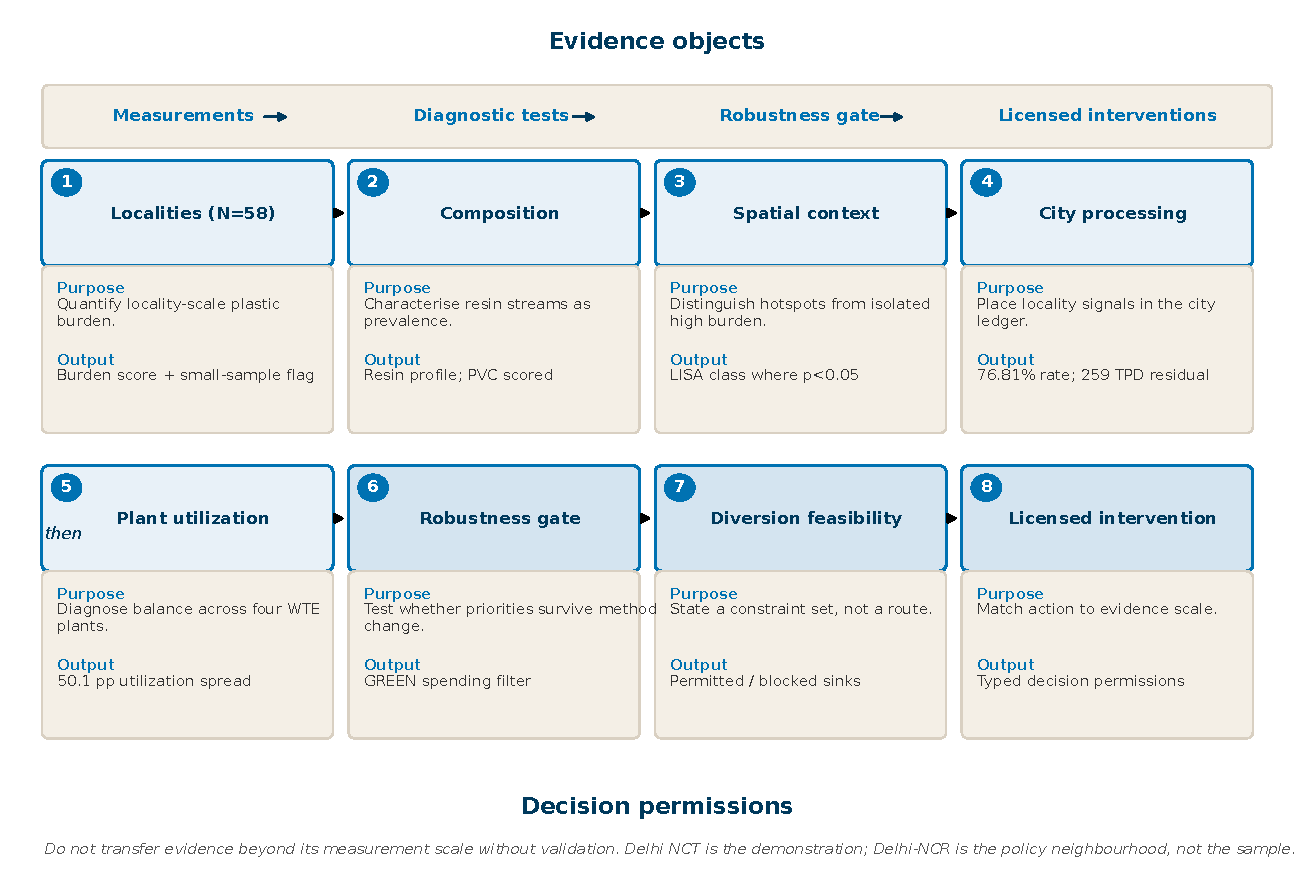
\includegraphics[width=\linewidth,keepaspectratio]{fig1.pdf}
\caption{Evidence-linked decision architecture. Top: evidence objects. Strip: measurements $\rightarrow$ diagnostic tests $\rightarrow$ robustness gate $\rightarrow$ licensed interventions. Bottom: decision permissions. An observation generated at one unit, extent, period, denominator, or system boundary is not transferred to a decision at another level without a demonstrated inference. Delhi NCT is the empirical demonstration; Delhi-NCR is the policy neighbourhood, not the sample. An optimal vehicle route is not claimed.}
\label{fig:fig1}
\end{figure}

%% ====================================================================
\section{Study Area and Empirical Data}
\label{sec:study_area_data}

This section defines the empirical boundary of the study and the provenance of the evidence objects used in the analysis. It first establishes the Delhi NCT sampling frame and then describes the city-level processing records, facility census, and supporting analytical files. The distinction between the measured NCT sample and the broader Delhi-NCR policy context is retained throughout.

\subsection{Geography and sampling frame}

Every locality, facility, and city-scale figure in this manuscript is from Delhi NCT: the sampled sites, the four WTE plants, and MCD spatial units. \emph{Delhi NCT empirical study area} means that measured geography. \emph{Delhi-NCR policy context} is reserved for Sections~\ref{sec:discussion} and~\ref{sec:implications}, where findings are offered as method, not as measured ranks, for districts outside NCT. Official Delhi sources used here --- the Economic Survey, MCD reporting, and CPCB affidavits \citep{delhi_eco_survey_2026,mcd_swm_ppt,ht_cpcb_affidavit_2026} --- likewise cover NCT/MCD jurisdiction only.

Plastic burden and resin composition were compiled for 58 Delhi NCT localities. Inclusion is defined by complete six-resin records in that compiled file: nothing is imputed, and sites outside the file are not represented. The 58 names are therefore the complete-case universe of the available locality file, not a probability sample of NCT neighbourhoods and not a census of MCD wards. The unit of inference is the sampled locality, not Delhi NCT as a statistically representative population. Delhi NCT contains far more named localities than this frame; land-use and income associations reported below are associations inside the file, not a claim that the file mirrors the territory. Four localities have waste samples below 10\,kg --- Kamla Nehru Ridge, DAV School, CBD Karkardooma, and Ryan International School --- and are retained with that flag rather than dropped. Zone, ward, and land-use context, where available, are drawn from the same frame. Local Moran's I is computed only for localities with valid coordinates under the $k=5$ nearest-neighbour weights specified in Section~\ref{sec:analytical_framework}; localities lacking that support are reported as not classified.

\subsection{City, facility, and provenance}

City-scale plastic generation and processing for Delhi NCT are taken from the Delhi Pollution Control Committee monthly progress reports submitted to the National Green Tribunal, Section VIII (Plastic Waste Management): 1,117 TPD generated and 858 TPD processed, recorded identically in the March 2025 and June 2025 reports \citep{dpcc_mpr_2025}. Those two reporting months are the two observations. Their ratio is a ledger entry, not a statistical estimate. No sampling distribution is available, so no confidence interval is reported, and the ratio is not used for trend, forecast, or significance testing. It is not comparable or additive to the Delhi Economic Survey 2025--26 total-MSW gap (approximately 4,200 TPD on approximately 11,862 TPD generated) \citep{delhi_eco_survey_2026,ht_delhi_63pct_2026}.

Utilization statistics for four Delhi NCT WTE facilities --- Ghazipur (1,300 TPD design), Tehkhand (2,000 TPD), Okhla (1,950 TPD), and Bawana (2,000 TPD) --- are taken from \citet{dpcc_mpr_2025}, \emph{Monthly Progress Report} for March 2025, Annexure-5. They are facility-level census snapshots for that reporting month, not a continuous operating series. Independent public reporting of downtime and compliance at these plants is used as external context in Section~\ref{sec:discussion} \citep{ht_ghazipur_shutdown_2026,ht_cpcb_affidavit_2026}.

All numerical results are taken from the locality composition file ($N=58$), the DPCC Section~VIII city plastic records and the four-plant Annexure-5 extract in \citet{dpcc_mpr_2025}, the robustness registry, the local Moran's I file, Kruskal--Wallis tests of income and land-use grouping, a Gini coefficient of spatial inequality, and Spearman correlations of burden with resin shares. Where an earlier draft conflicted with these files, the file value was kept. Table~\ref{tab:provenance} states the evidence objects, units, periods, and limitations that prevent those files from being averaged into a single circularity score. Table~\ref{tab:table1} summarizes the sampling universe used throughout. The order of those layers is shown in Figure~\ref{fig:fig1}.

\begin{table}[htbp]
\centering
\caption{Data provenance: evidence objects kept on separate ledgers}
\label{tab:provenance}
\resizebox{\textwidth}{!}{%
\begin{tabular}{L{2.4cm}L{1.8cm}L{2.2cm}L{0.8cm}L{2.4cm}L{2.4cm}L{3.0cm}}
\toprule
\textbf{Evidence} & \textbf{Unit} & \textbf{Period} & \textbf{N} & \textbf{Source} & \textbf{Role} & \textbf{Main limitation} \\
\midrule
Plastic burden and resin mix & Locality & Compiled complete-resin file & 58 & Locality composition file & Object A: burden and prevalence & Complete-case frame, not a probability sample; four sites $<$10\,kg \\
Spatial association & Locality (coordinates) & Same frame & 58 & Local Moran's I file & Object B: cluster vs isolated peak & Exploratory site-wise $p$; no FDR; unclassified $\neq$ low burden \\
City plastic ledger & Delhi NCT & March and June 2025 & 2 & DPCC MPR Section VIII \citep{dpcc_mpr_2025} & Object C: processed/generated ratio & Two records; no interval; no trend \\
WTE utilization & Facility & March 2025 census & 4 & DPCC MPR Annexure-5 \citep{dpcc_mpr_2025} & Object D: utilization class and mixed-waste headroom & Snapshot, not continuous availability; mixed-waste, not plastic \\
Priority stability & Locality rank & Specification registry & 72 rows & Robustness file & Object E: GREEN/AMBER/RED gate & Gate, not a score; mean $\rho$ does not licence every name \\
Diversion feasibility & Origin--sink pair & Scenario, not a timetable & -- & Utilization classes + GREEN demand & Object F: constraint set & No GPS, fleet, time windows, or costs \\
\bottomrule
\end{tabular}%
}
\begin{flushleft}
\footnotesize\textit{Note.} Objects are linked sequentially, not averaged. External reports (Economic Survey, CPCB affidavit, shutdown coverage) are context, convergence, or contrast and never override these files.
\end{flushleft}
\end{table}



\begin{table}[htbp]
\centering
\caption{Empirical data coverage and material-composition baseline}
\label{tab:table1}
\resizebox{\textwidth}{!}{%
\begin{tabular}{L{2.6cm}L{1.8cm}L{0.8cm}L{1.6cm}L{1.0cm}L{1.1cm}L{3.4cm}L{1.0cm}L{1.7cm}L{2.2cm}}
\toprule
\textbf{Variable} & \textbf{Obs.\ level} & \textbf{N} & \textbf{Mean} & \textbf{SD} & \textbf{Min} & \textbf{Max} & \textbf{Unit} & \textbf{Data source} & \textbf{Analytical role} \\
\midrule
Sampled localities & Locality & 58 & -- & -- & -- & -- & count & Locality composition file & Complete-case frame, not a census \\
Complete resin cases & Locality & 58 & -- & -- & -- & -- & count & Locality composition file & Basis for composition analysis \\
Small-sample flag ($<$10\,kg) & Locality & 4 & -- & -- & -- & -- & count & Field sample mass & Ridge, DAV School, CBD Karkardooma, Ryan International; retained, not dropped \\
Plastic \% & Locality & 58 & 10.82 & 6.10 & 1.98 (Okhla Mandi) & 30.49 (Kamla Nehru Ridge) & \% & Locality composition file & Basis for burden score \\
PET \% & Locality & 58 & 23.60 & 20.27 & 0.95 & 100.00 (Akshardham Temple) & \% & Locality composition file & Descriptive composition indicator \\
PP \% & Locality & 58 & 2.79 & 6.54 & 0.00 & 34.67 (Kamla Nehru Ridge) & \% & Locality composition file & Descriptive composition indicator \\
HDPE/LDPE \% & Locality & 58 & 53.24 & 24.49 & 0.00 & 95.28 (Shakarpur) & \% & Locality composition file & Descriptive composition indicator \\
PS \% & Locality & 58 & 4.92 & 6.69 & 0.00 & 36.45 (Ryan International) & \% & Locality composition file & Descriptive composition indicator \\
PVC \% & Locality & 58 & 1.65 & 2.41 & 0.00 & 15.43 (DAV School) & \% & Locality composition file & Scored problematic-material indicator \\
Others \% & Locality & 58 & 13.80 & 13.17 & 0.00 & 45.63 (Chanakyapuri) & \% & Locality composition file & Residual descriptive category \\
\bottomrule
\end{tabular}%
}
\begin{flushleft}
\footnotesize\textit{Note.} Burden score is plastic \% divided by the sample maximum (Kamla Nehru Ridge = 30.49\% = 1.000). It is a relative index inside this $N=58$ frame, not an absolute environmental-risk score. PET and PP are descriptive composition indicators; PVC is a scored problematic-material indicator. Four sites have sample mass below 10\,kg and are flagged in the text. The 58 names are the complete-resin cases in the locality composition file, not a probability sample of Delhi NCT.
\end{flushleft}
\end{table}

%% ====================================================================
\section{Analytical Framework}
\label{sec:analytical_framework}

The analytical framework converts the evidence boundary defined above into a sequential decision procedure. It first defines the evidence objects and the rule governing transfer between analytical scales, then specifies the burden, spatial, processing, utilization, robustness, and feasibility procedures. The final stage translates surviving evidence into intervention permissions without combining the layers into a single circularity score.

\subsection{Evidence objects}

Six evidence objects are reported on their own terms rather than being combined into a single composite score. Object A is locality material burden and composition. Object B is spatial association. Object C is the city processing ledger. Object D is facility utilization. Object E is robustness classification. Object F is the intervention constraint set. They are linked sequentially, not averaged. The sequential hand-off is required because each object answers a different operational question; averaging them would recreate the mismatch the architecture is designed to prevent. Table~\ref{tab:terminology} is the glossary: a term marked scored enters ranking; a term marked descriptive does not. Table~\ref{tab:provenance} states the unit, period, and limitation of each object. Robustness (Object E) is a gate applied to locality ranks (Object A). It is not mixed into Objects A--D as an extra score. Every major Results and Discussion claim states the internal observation with file provenance, hedges the interpretation, identifies the best available external evidence (Tier 1: CPCB, MoEFCC, MCD, PIB/Government of India; Tier 2: peer-reviewed or World Bank; Tier 3: reputable news, used only for recent plant events), names at least one mismatch of denominator, unit, period, or geography, and commits only to wording the design can defend. External evidence is context, convergence, or contrast. It never overrides the primary files. The matching claim-boundary is stated once at the opening of Section~\ref{sec:results}; defended claims are translated into the intervention screen later in the Results.



\begin{table}[htbp]
\centering
\caption{Terminology used for each evidence layer}
\label{tab:terminology}
\begin{tabular}{L{4.0cm}L{9.7cm}}
\toprule
\textbf{Term} & \textbf{Meaning as used in this manuscript} \\
\midrule
Plastic burden indicator (scored) & Locality plastic \% and its 0--1 normalized burden score (Kamla Nehru Ridge = 1.000 within $N=58$). \\
PVC problematic-material indicator (scored) & Locality PVC \%; higher values indicate higher problematic-material burden, scored only where the underlying data are validated. \\
PET composition indicator (descriptive) & Locality PET \%, read as PET prevalence relevant to recovery assessment, never as realized recycling, material quality, or collection efficiency, and never scored as a circularity outcome. \\
PP composition indicator (descriptive) & Locality PP \%, read as packaging prevalence context. E-commerce relevance is interpretive, not directly measured, and PP is not scored as a performance outcome. \\
HDPE/LDPE, PS, Others (descriptive) & Compositional shares reported for completeness; not independently scored. \\
City plastic processing performance indicator & Processed/generated plastic tonnage ratio at Delhi NCT scale (two recorded TPD figures); a ledger ratio, not a statistical estimate. \\
WTE infrastructure utilization & Processed/designed-capacity ratio per facility (4 facilities; March 2025 census snapshot). \\
Spatial context & Zone, ward, land use, and local cluster classification per locality, confined to the Delhi NCT study area. \\
Robust intervention priority & A locality whose recorded class is GREEN (Section~\ref{sec:res-robust}). Immediate collection spend is licensed only for those names. Robustness is a gate and a classification, not an additional score. \\
Typed intervention licence & A decision permission whose spatial and operational scope matches the evidence object that supports it: site, zone, facility, city investigation, or later optimization (Table~\ref{tab:licensed}). \\
Evidence-scale mismatch & Use of an observation generated at one analytical unit, geographic extent, temporal window, denominator, or system boundary to justify a decision at another level without demonstrating that the inference is transferable (Table~\ref{tab:mismatch}). \\
Licensed intervention & An action that operates at the same decision scale as the supporting evidence, states its uncertainty, and does not require an unmeasured causal or operational assumption (Table~\ref{tab:licensed}). \\
\bottomrule
\end{tabular}
\end{table}

\subsection{Evidence-scale mismatch and the licensing rule}

The architecture does not combine layers into a circularity score. It asks which policy decision is licensed by a particular observation, at a particular scale, under the recorded limitations. Evidence-scale mismatch is defined as the use of an observation generated at one analytical unit, geographic extent, temporal window, denominator, or system boundary to justify a decision at another level without demonstrating that the inference is transferable. Table~\ref{tab:mismatch} names five forms of that mismatch and illustrates each with an object already present in this study. The sequence that follows is therefore:

\[
\text{evidence unit}
\rightarrow
\text{permitted inference}
\rightarrow
\text{decision scale}
\rightarrow
\text{robustness}
\rightarrow
\text{licensed intervention.}
\]

An intervention is evidence-licensed only when the proposed action operates at the same decision scale as the supporting evidence, its uncertainty is stated, and no unmeasured causal or operational assumption is required. Table~\ref{tab:licensed} applies that rule to the Delhi NCT objects used later in the results. The table is a reading rule, not a claim that the architecture has been shown to prevent bad decisions in live systems. The recorded decision rule is:

\begin{equation}
L_i =
\begin{cases}
\text{Intervention}, & \text{if the recorded class is GREEN and the action matches the evidence scope}\\
\text{Investigation}, & \text{if the evidence is informative but AMBER, incomplete, or off-scope for spend}\\
\text{Withhold}, & \text{if the recorded class is RED or the proposed action requires an unmeasured transfer.}
\end{cases}
\end{equation}

This is a classification rule, not a fitted model. The Investigation and Withhold branches are not a failure of ranking. They are the defensible response when the evidence is informative but unstable, incomplete, or scoped to a different decision. Forcing a complete priority list from such evidence would convert uncertainty into an unearned spending claim.

\begin{table}[htbp]
\centering
\caption{Five forms of evidence-scale mismatch}
\label{tab:mismatch}
\begin{tabular}{L{2.6cm}L{6.2cm}L{5.0cm}}
\toprule
\textbf{Form} & \textbf{What is transferred without warrant} & \textbf{Delhi NCT illustration in this study} \\
\midrule
Spatial mismatch & Locality evidence used to make citywide or NCR-wide claims & $N=58$ complete-resin localities are not a probability sample of NCT neighbourhoods and not a census of MCD wards; Delhi-NCR is not sampled \\
Temporal mismatch & A two-time-point processing estimate used to imply a long-term trend & DPCC Section~VIII records 1,117 TPD generated and 858 TPD processed in March and June 2025; $N=2$, no interval, no trend \\
Material mismatch & PET/PP composition used as evidence of actual material recovery & Mean PET 23.60\% is prevalence relevant to recovery assessment, not locality PET capture \\
System-boundary mismatch & Plastic-specific processing compared directly with total-MSW processing & 76.81\% plastic processed ($858/1{,}117$) is a different denominator from $\approx$63\% total MSW processed \\
Operational mismatch & WTE utilization or benchmark headroom treated as immediate routing capacity or optimized flow allocation & Combined mixed-waste headroom of 688.4 TPD is not plastic-only capacity, not continuous availability, and not a solved route \\
\bottomrule
\end{tabular}
\end{table}

\begin{table}[htbp]
\centering
\caption{Evidence, licensed intervention, and the claim the evidence does not support}
\label{tab:licensed}
\resizebox{\textwidth}{!}{%
\begin{tabular}{L{3.4cm}L{5.0cm}L{5.4cm}}
\toprule
\textbf{Evidence} & \textbf{Licensed intervention} & \textbf{Not licensed} \\
\midrule
High locality plastic burden (Ridge 30.49\%; Kashmere Gate ISBT 30.25\%; CBD Karkardooma 22.68\%) & Enhanced collection and segregation assessment at surviving GREEN names & Claiming citywide processing failure from locality shares \\
High PET composition (mean 23.60\%; Kashmere Gate ISBT 83.68\%) & MRF access and recovery audit where PET is prevalent & Claiming high PET circularity or locality recovery \\
High PVC at DAV School (15.43\%) & Site-level material investigation & Citywide PVC restriction \\
Underutilized Ghazipur (58.3\%) and Tehkhand (68.0\%) & Feasibility assessment for diversion up to mixed-waste headroom & Immediate guaranteed diversion allocation or a solved route \\
Bawana at 108.4\% utilization & Operational-relief assessment; keep Okhla (95.8\%) as High Utilization, not slack & Claiming a proven cause of emissions non-compliance \\
Robust top locality rank (three of 58 names; $\rho=0.893$) & Priority field intervention at Ridge, Kashmere Gate ISBT, and CBD Karkardooma & Claiming a causal explanation for their burden, or treating untested ranks as a programme \\
\bottomrule
\end{tabular}%
}
\begin{flushleft}
\footnotesize\textit{Note.} An intervention is evidence-licensed only when the action operates at the same decision scale as the supporting evidence, uncertainty is stated, and no unmeasured causal or operational assumption is required. Read with the mismatch typology. The later intervention screen applies the same rule.
\end{flushleft}
\end{table}




\subsection{Plastic burden and resin composition}

Plastic burden is the observed plastic percentage at each locality within the $N=58$ sample, rescaled to a 0--1 score against the sample maximum (Kamla Nehru Ridge $=1.000$). That score is intentionally descriptive and relative to this study frame; it is not an absolute environmental-risk score, a z-score, or an externally defined threshold. Four small-sample sites are scored with that flag attached. Resin composition is the percentage share of PET, PP, HDPE/LDPE, PS, PVC, and Others on the same file; these shares are compositional and sum to 100\% at each locality. PVC is treated as a scored problematic-material indicator. PET and PP are reported as descriptive composition indicators; they are not converted into a circularity score. PET is read as prevalence relevant to recovery assessment, not as recyclability of the sampled material. The named-locality sheet and the corresponding ranking plot are given in Table~\ref{tab:table2} and Figure~\ref{fig:fig2}.

\subsection{Spatial heterogeneity and local cluster analysis}

Locality-level plastic burden is mapped against available zone, ward, and land-use context. Local Moran's I is computed only for localities with valid latitude--longitude coordinates. Because the observations are irregular point sites rather than a closed polygon lattice, queen or rook contiguity is not defined. The spatial weights matrix is therefore a $k$-nearest-neighbour specification with $k=5$, using great-circle (Haversine) distance in kilometres, inverse-distance weights among those five neighbours, and row-standardization so that each site's weights sum to one \citep{anselin_lisa_1995}. Global Moran's I uses the same weights. Local Moran's I and a pseudo $p$-value from 999 conditional permutations are then computed at each site, following the hotspot/outlier reading used for Indian MSW at ward scale \citep{getis_ord_1992,ieam_kota_landuse_msw_2026} but applied here to locality plastic burden. Those local tests are treated as exploratory: a family-wise or false-discovery correction is not applied across the 58 sites, so $p<0.05$ is a site-wise permutation threshold, not a citywide error rate. Ajmal Khan Road Market ($0.05\leq p<0.10$) is reported as marginal and is not treated as a confirmed cluster. Cluster classifications are reported only where the statistic and $p$-value are available. A Gini coefficient is computed as a descriptive inequality metric on the same frame, without an external ``moderate''/``high'' threshold. Cluster labels, local Moran's I statistics, and the high-burden versus hotspot split are recorded in Table~\ref{tab:table3} and mapped in Figure~\ref{fig:fig3}. Localities without a significant LISA class are treated as not classified, not as low-burden.

\subsection{City processing and plant utilization}

Processing performance is processed tonnage divided by generated tonnage on the two DPCC Section~VIII records \citep{dpcc_mpr_2025}. With only two observations, no interval is computed. That ratio is compared descriptively with an 85\% operating-band reference. The 85\% figure is not a SWM Rules target and is not a CPCB regulatory threshold. It is the lower edge of this manuscript's plant-classification scheme: 100\% is design capacity, the hard physical bound; 85\% leaves a 15~percentage-point buffer for outages and maintenance, which the reported 108-day Ghazipur shutdown shows is not a hypothetical risk \citep{ht_ghazipur_shutdown_2026}. Facility utilization is processing volume divided by designed capacity at each of the four plants, classed as Underutilized ($<$85\%), Optimal (85--95\%), High Utilization (95--100\%, below design and not treated as slack), or Over-Stressed ($>$100\%). Headroom to 85\% is additional mixed-waste throughput to that operating band, not plastic-only capacity and not unconstrained spare capacity to 100\% of design. The city ratio is recorded in Table~\ref{tab:table4} and Figure~\ref{fig:fig4}; band assignments and mixed-waste headroom are set out in Table~\ref{tab:table5} and Figure~\ref{fig:fig5}.

\subsection{Robustness testing of locality priorities}

Locality-level intervention priorities are tested against the recorded robustness registry: six weighting tests, three normalization tests, 58 leave-one-out removals, one missing-data comparison, and four facility-benchmark tests (72 specification rows in total). The perturbations were chosen to challenge three potential sources of ranking instability: criterion importance, scale transformation, and individual-observation influence. Weighting tests vary criterion importance; normalization tests vary scale transformation; leave-one-out removals vary observation influence. Robustness is a gate and a classification, not an additional score. The gate is necessary because a high mean rank correlation can coexist with unstable decision units; without it, an untested top-10 would be treated as a programme. It is evaluated relative to the proposed intervention (Table~\ref{tab:robusttests}). Two properties are scored separately. Appearance stability asks whether the locality remains in the recorded top-10 when weights and scaling change. Leave-one-out influence asks whether removing that locality rearranges the remaining names. GREEN requires both: the name survives specification change, and it does not distort the ranking of other names. Leave-one-out influence is therefore material when the proposed action is a cross-locality programme. It does not by itself disqualify a site-specific collection action at a locality whose own removal moves remaining ranks by about one position.

The recorded classes follow that rule. GREEN requires appearance in at least 8 of 9 recorded top-10 weighting/normalization tests (88.9\%) and the absence of leave-one-out influence, defined in the registry as mean displacement of remaining ranks greater than 1.0 when the locality is removed. Kamla Nehru Ridge, Kashmere Gate ISBT, and CBD Karkardooma meet both conditions (appearance 8/9; mean leave-one-out displacement 0.98, 0.96, and 0.95, with maxima of 2, 1, and 1). Immediate site collection is therefore licensed at those generators within the study's decision rule. DAV School records 9/9 appearance but is AMBER because removing it shifts other ranks by a mean of 3.7 positions (maximum 19). That is leave-one-out influence: it would not support a multi-site PVC programme, and the licensed action at DAV School is therefore a site investigation. AMBER otherwise denotes evidence stable enough for investigation but not for immediate allocation (National Museum 7/9; Shakarpur 6/9). RED denotes a conclusion that depends materially on specification (Ryan International School, 5/9). Most names in the file do not survive that gate. GREEN/AMBER/RED apply only to locality priorities. They are not reused as labels for plants, spatial clusters, or city ledgers. Appearance rates and leave-one-out influence are collected in Table~\ref{tab:table6} and Figure~\ref{fig:fig6}.

\begin{table}[htbp]
\centering
\caption{Robustness tests and the intervention each one can affect}
\label{tab:robusttests}
\begin{tabular}{L{3.4cm}L{5.4cm}L{5.0cm}}
\toprule
\textbf{Test} & \textbf{What it protects against} & \textbf{Intervention affected} \\
\midrule
Appearance stability ($\geq$8/9 top-10 tests) & Whether the locality remains in the recorded top-10 when weights and scaling change & Site-priority licence (GREEN if also not LOO-influential) \\
Leave-one-out influence (mean displacement of remaining ranks $>1.0$) & Effect of removing a locality on the ranking of the remaining localities & Multi-site programme; not a bar to site collection at a non-influencer \\
\bottomrule
\end{tabular}
\begin{flushleft}
\footnotesize\textit{Note.} Kashmere Gate ISBT is GREEN: 8/9 appearance and mean leave-one-out displacement 0.96 (maximum 1). DAV School is AMBER: 9/9 appearance but mean displacement 3.7 (maximum 19). The threshold mean $>1.0$ is the registry rule used to flag influential removals.
\end{flushleft}
\end{table}

\subsection{Scenario-based diversion constraint set}

Facility-wise utilization is the supply-chain layer of the design. Plants below 85\% of design become candidate sinks up to mixed-waste headroom at that operating band. Plants between 85\% and 100\% of design are retained as conditionally admissible, subject to operating and compliance checks, and are not treated as slack. An over-stressed plant ($>$100\% of design) is a blocked node. The current files therefore provide origins, candidate sinks, and capacity constraints. They do not provide network topology, fleet, time windows, or costs. The constraint set is necessary because a utilization class is not yet a route: it states which nodes may receive additional load, and which must not. Joined to surviving locality burden, those classes specify a constraint set for later routing, not a solved timetable: high-burden sites as demand nodes, Ghazipur and Tehkhand as candidate sinks, Bawana as a blocked node. Catchments and GPS hauls are not observed. A capacitated vehicle-routing or network-flow model can inherit this file once road, fleet, and time-window data exist; that model is reserved as future work.

\subsection{What can be reused, and what cannot}
\label{sec:transfer}

The $N=58$ localities and the two-point processing ledger are described in Section~\ref{sec:study_area_data}. What can be reused is the sequence of evidence layers --- locality, city, and facility kept separate; composition read as prevalence until capture is measured; plants classed from a utilization census snapshot before a capacity shortage is announced; a high plastic share distinguished from a confirmed cluster; any priority list passed through a specification registry; intervention licensed only at the scale of the supporting evidence. A city that has those files can run the same sequence. It cannot import these ranks, these three surviving names, or the two-point processing ratio. The architecture can travel; its practical performance in cities with different governance, collection, informal-sector, and treatment configurations remains to be tested. Delhi results remain specific to the sampled NCT localities and the observed periods.

%% ====================================================================
\section{Results}
\label{sec:results}

Results follow the same architecture: material burden and composition (Section~\ref{sec:res-burden}); spatial diagnosis (Section~\ref{sec:res-spatial}); city processing and plant utilization (Section~\ref{sec:res-processing}); the robustness gate (Section~\ref{sec:res-robust}); and the reverse-logistics constraint set together with the intervention screen (Section~\ref{sec:res-routing}). Table~\ref{box:cancannot} is the first results object; subsequent findings are read against that boundary and against the licensing rule in Table~\ref{tab:licensed}.



\begin{table}[htbp]
\centering
\caption{What the data establish and do not establish}
\label{box:cancannot}
\begin{tabular}{L{7.2cm}L{7.2cm}}
\toprule
\textbf{Established by this study} & \textbf{Not established by this study} \\
\midrule
Locality-level plastic burden ($N=58$) & Locality-level PET recovery rate \\
Resin composition by category ($N=58$) & Locality-level PP recovery rate \\
Spatial variation across sampled Delhi NCT localities; LISA hotspots where $p<0.05$ & Causal effect of land use on plastic burden; citywide hotspot map for unclassified points \\
City-level plastic processing ratio (two recorded TPD figures; no interval) & Causal impact of EPR enforcement on Delhi outcomes \\
WTE facility utilization differences (4 facilities, census) & Complete Delhi-NCR coverage \\
Robustness of priority rankings (appearance-rate and LOO tests) & Continuous WTE plant availability from one utilization estimate \\
Benchmark-based facility headroom scenarios & Mathematically optimal vehicle routes \\
\bottomrule
\end{tabular}
\end{table}




\subsection{Plastic burden and resin composition}
\label{sec:res-burden}

\textbf{Finding.} Plastic burden varied substantially inside the available frame. \textbf{Quantification.} Across 58 complete-resin localities it ranged from 1.98\% at Okhla Mandi to 30.49\% at Kamla Nehru Ridge (burden score 1.000), with Kashmere Gate ISBT at 30.25\% (0.992) and CBD Karkardooma at 22.68\% (0.744) (Table~\ref{tab:table1}; Table~\ref{tab:table2}; Figure~\ref{fig:fig2}). HDPE/LDPE dominated the mean composition (53.24\%), followed by PET (23.60\%). DAV School exhibited the highest PVC share (15.43\%), while Kashmere Gate ISBT and Shakarpur were unusually PET-rich (83.68\%) and HDPE/LDPE-rich (95.28\%), respectively. \textbf{Interpretation boundary.} These are prevalence observations within $N=58$, not recovery measurements and not a citywide census. Four sites are small-sample flags ($<$10\,kg), not deletions. Spearman correlations of plastic burden with PET, HDPE/LDPE, PVC, PP, and PS shares are not significant after FDR correction. \textbf{Decision consequence.} The upper tail is a candidate for site screening, subject to the robustness gate; PET prevalence licences a capture/MRF assessment, not a circularity claim; the PVC spike licences a site investigation, not a citywide restriction. The range matters because a citywide composition mean would not name the generators a collection contract has to serve.



\begin{table}[htbp]
\centering
\caption{Locality-level plastic burden and resin composition ($N=58$; selected localities shown)}
\label{tab:table2}
\resizebox{\textwidth}{!}{%
\begin{tabular}{L{2.6cm}L{1.4cm}L{1.5cm}L{1.2cm}L{1.2cm}L{1.1cm}L{1.5cm}L{1.0cm}L{1.3cm}L{2.0cm}}
\toprule
\textbf{Locality} & \textbf{Plastic \%} & \textbf{Burden score} & \textbf{PVC \%} & \textbf{PET \%} & \textbf{PP \%} & \textbf{HDPE/ LDPE \%} & \textbf{PS \%} & \textbf{Others \%} & \textbf{Robustness} \\
\midrule
Kamla Nehru Ridge & 30.49 & 1.000 & 0.00 & 6.67 & 34.67 & 58.67 & 0.00 & 0.00 & GREEN (small sample) \\
Kashmere Gate ISBT & 30.25 & 0.992 & 0.00 & 83.68 & 0.00 & 9.30 & 0.00 & 7.02 & GREEN \\
CBD Karkardooma & 22.68 & 0.744 & 0.00 & 38.58 & 0.00 & 30.71 & 16.54 & 14.17 & GREEN (small sample) \\
National Museum & 19.51 & 0.640 & 0.00 & 52.10 & 0.00 & 47.90 & 0.00 & 0.00 & AMBER \\
Ryan International School & 19.11 & 0.627 & 0.00 & 19.63 & 0.00 & 43.93 & 36.45 & 0.00 & RED \\
DAV School & 17.24 & 0.565 & 15.43 & 14.04 & 16.01 & 41.76 & 12.76 & 0.00 & AMBER (LOO influential) \\
Shakarpur & 17.10 & 0.561 & 0.80 & 0.95 & 0.00 & 95.28 & 2.17 & 0.80 & AMBER \\
\multicolumn{10}{l}{\textit{Remaining 51 of 58 localities: same composition file; ranked list not reprinted here.}} \\
\bottomrule
\end{tabular}%
}
\begin{flushleft}
\footnotesize\textit{Note.} Burden score = plastic \% / 30.49. PVC is scored; PET, PP, HDPE/LDPE, PS, and Others are descriptive. Small-sample sites ($<$10\,kg): Ridge, DAV School, CBD Karkardooma, Ryan International. Robustness categories are assigned in the later robustness registry.
\end{flushleft}
\end{table}






\begin{figure}[htbp]
\centering
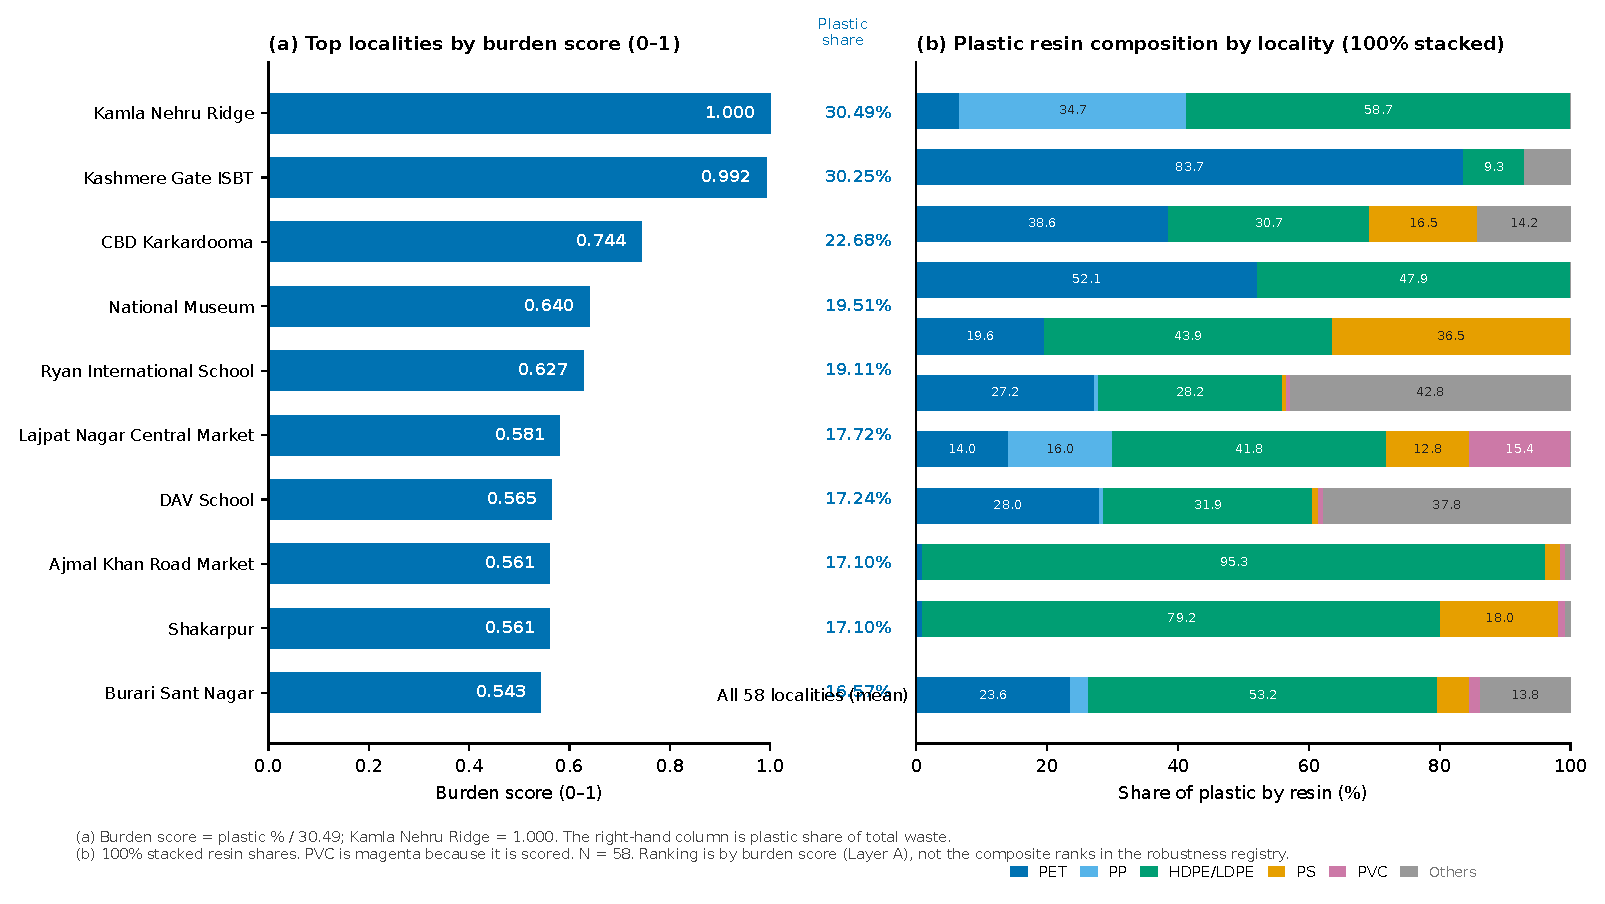
\includegraphics[width=\linewidth,keepaspectratio]{fig2.pdf}
\caption{Locality burden and resin composition ($N=58$). Panel (a) ranks the top ten localities by plastic-burden score (Layer A); Kashmere Gate ISBT $=0.992$. Panel (b) is compositional prevalence, not recovery. This ranking is not the later composite-priority ranking. Data: locality composition file.}
\label{fig:fig2}
\end{figure}




\subsection{Spatial heterogeneity}
\label{sec:res-spatial}

\textbf{Finding.} High burden did not imply spatial clustering. \textbf{Quantification.} Kruskal--Wallis tests with FDR correction show a significant association of plastic share with income level ($H=14.00$, $\varepsilon^2=0.208$, $q=0.012$) and with land-use type ($H=14.83$, $\varepsilon^2=0.193$, $q=0.022$); PVC share is not significantly associated with either grouping. Spatial inequality of plastic burden within the sampled frame is Gini $=0.301$; PVC share is more concentrated (Gini $=0.586$). Global Moran's I is consistent with a random pattern ($I=0.053$). Local Moran's I under $k=5$ nearest-neighbour, row-standardized inverse-distance weights and 999 permutations nevertheless marks local structure (Table~\ref{tab:table3}; Figure~\ref{fig:fig3}): Kamla Nagar Market and Tis Hazari Court were significant high--high clusters ($p=0.002$ and $p=0.028$), whereas Kamla Nehru Ridge and Kashmere Gate ISBT, despite occupying the extreme burden tail, were not significant LISA hotspots. Madanpur Khadar and Dwarka Sector-12 are low--low coldspots; Civil Lines is a low--high outlier and Nizamuddin Railway Station a high--low outlier. \textbf{Interpretation boundary.} Those coefficients describe unequal distribution inside $N=58$. A burden ranking and a spatial intervention map therefore answer different questions. \textbf{Decision consequence.} Confirmed high--high clusters licence zone attention; isolated high-burden generators licence site lifting only after the robustness gate. That split matters because treating an isolated generator as a zone, or a confirmed cluster as a single site, would apply the wrong operational object.



\begin{table}[htbp]
\centering
\caption{Spatial heterogeneity and locality-level priority evidence}
\label{tab:table3}
\resizebox{\textwidth}{!}{%
\begin{tabular}{L{2.4cm}L{1.2cm}L{1.1cm}L{1.6cm}L{1.5cm}L{2.0cm}L{0.9cm}L{1.7cm}L{2.6cm}}
\toprule
\textbf{Locality} & \textbf{Ward} & \textbf{Zone} & \textbf{Land use} & \textbf{Plastic burden} & \textbf{Spatial statistic (local Moran's I)} & \textbf{p} & \textbf{Cluster class.} & \textbf{Interpretation} \\
\midrule
Kamla Nagar Market & 69 & North & Commercial & 15.00 & 2.183 & 0.002 & High--high & Strong hotspot \\
Tis Hazari Court & 83 & North & Institutional & 11.53 & 0.119 & 0.028 & High--high & Strong hotspot \\
Madanpur Khadar & 101-S & South East & Residential & 5.30 & 0.949 & 0.006 & Low--low & Strong coldspot \\
Dwarka Sector-12 & 36 \& 38 & Dwarka & Residential & 9.27 & 0.228 & 0.028 & Low--low & Strong coldspot \\
Civil Lines & 83 & North & Residential & 6.75 & $-$2.157 & 0.040 & Low--high & Spatial outlier \\
Nizamuddin Railway Station & -- & South East & Public & 11.13 & $-$0.060 & 0.040 & High--low & Spatial outlier \\
Kamla Nehru Ridge & Ridge & Central & Mixed & 30.49 & -- & -- & Not classified & Highest burden; not a LISA hotspot \\
Kashmere Gate ISBT & -- & North & Public & 30.25 & -- & -- & Not classified & Isolated high-burden generator \\
\bottomrule
\end{tabular}%
}
\begin{flushleft}
\footnotesize\textit{Note.} Spatial weights: $k=5$ nearest neighbours (Haversine km), inverse-distance among those neighbours, row-standardized. Local Moran's I from 999 conditional permutations; site-wise $p<0.05$ labelled strong. No false-discovery correction is applied across the 58 local tests; classifications are exploratory. Ajmal Khan Road Market is a marginal high--high cluster ($p=0.066$) and is not treated as confirmed. High-burden GREEN sites without a LISA label are isolated generators, not hotspots. Method follows ward-level MSW hotspot analysis in \citep{ieam_kota_landuse_msw_2026}, adapted to locality plastic burden. Delhi NCT sample only.
\end{flushleft}
\end{table}






\begin{figure}[htbp]
\centering
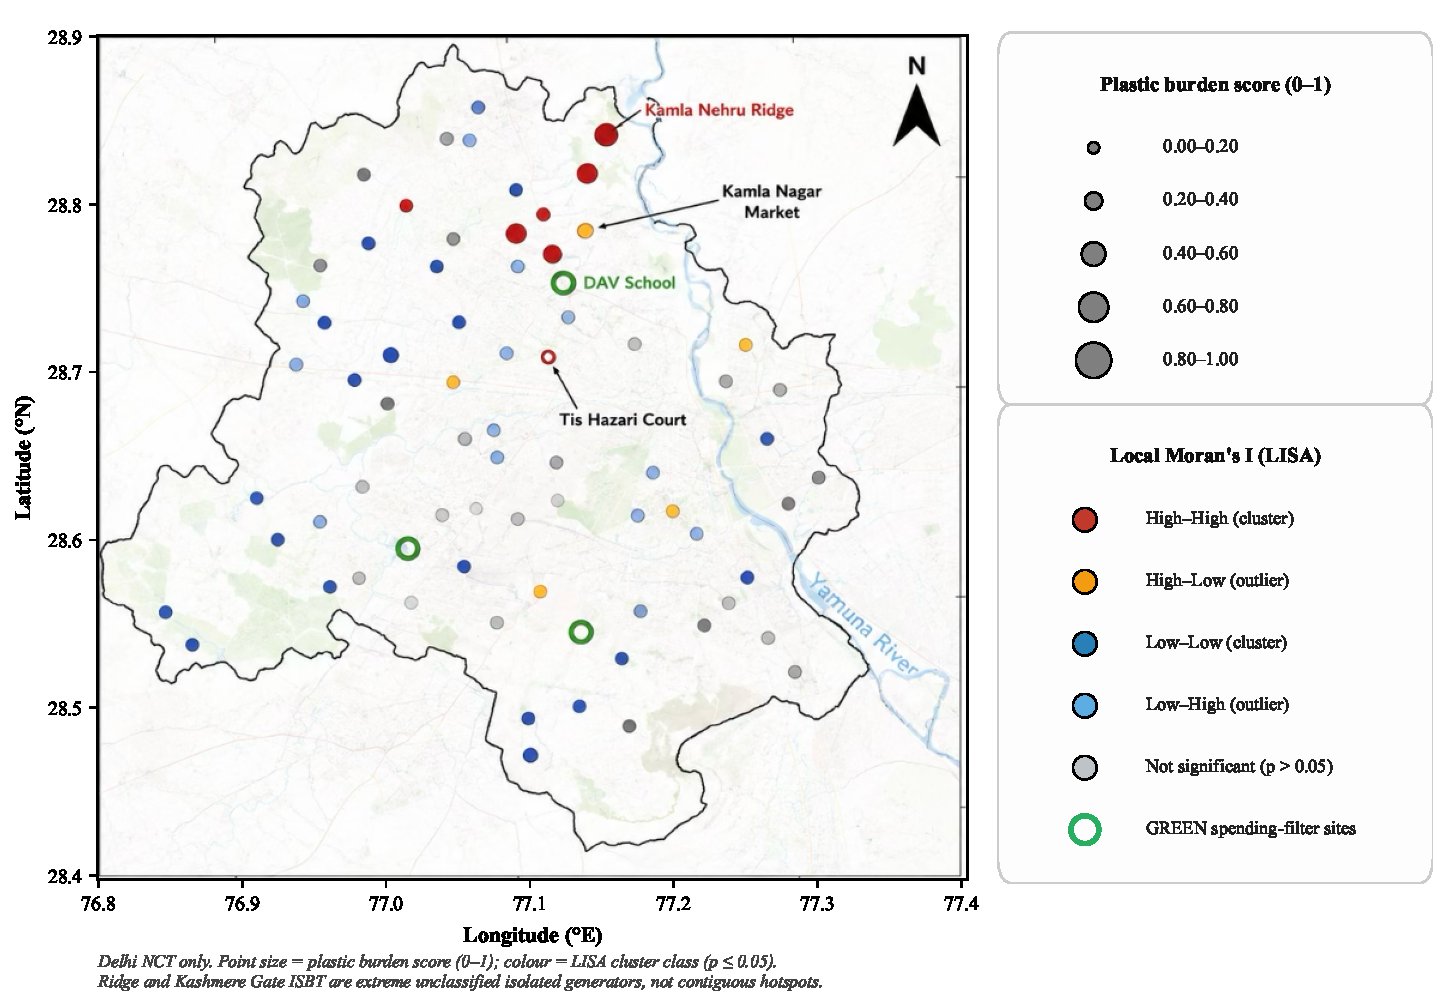
\includegraphics[width=\linewidth,keepaspectratio]{fig3.pdf}
\caption{Spatial pattern of plastic burden and local Moran's I inside Delhi NCT ($N=58$). Point size is burden score; colour is LISA class where $p\leq 0.05$. GREEN rings mark the three names later licensed for immediate spend: Kamla Nehru Ridge, Kashmere Gate ISBT, and CBD Karkardooma. No NCR districts are mapped.}
\label{fig:fig3}
\end{figure}




\subsection{City processing and plant utilization}
\label{sec:res-processing}

\textbf{Finding.} City-scale plastic processing is a two-record ledger, not a trend, and it does not diagnose which plant is constrained. \textbf{Quantification.} DPCC Section~VIII records 1,117 TPD generated against 858 TPD processed, identically in March 2025 and June 2025, or 76.81\%, with an arithmetic remainder of 259 TPD (Table~\ref{tab:table4}; Figure~\ref{fig:fig4}). \textbf{Interpretation boundary.} With only two recorded quantities, no interval accompanies the ratio. It is not comparable with the Economic Survey 2025--26 figure of about 63\% total MSW processed, because the denominators differ \citep{delhi_eco_survey_2026,ht_delhi_63pct_2026}. \textbf{Decision consequence.} The ledger licences a plastic line and a fate investigation. It does not licence a plant-capacity claim. A city processing ratio cannot name which grate is slack or over-run; that is why the next object is a facility census rather than a capacity announcement.



\begin{table}[htbp]
\centering
\caption{Delhi NCT plastic processing performance}
\label{tab:table4}
\resizebox{\textwidth}{!}{%
\begin{tabular}{L{3.4cm}L{1.8cm}L{1.4cm}L{2.2cm}L{1.7cm}L{2.2cm}L{3.2cm}}
\toprule
\textbf{Metric} & \textbf{Value} & \textbf{Unit} & \textbf{Benchmark} & \textbf{Difference} & \textbf{Evidence source} & \textbf{Interpretation} \\
\midrule
Estimated generation & 1,117 & TPD & -- & -- & DPCC MPR, March and June 2025, Section VIII \citep{dpcc_mpr_2025} & Identical in both months \\
Processed & 858 & TPD & -- & -- & DPCC MPR, March and June 2025, Section VIII \citep{dpcc_mpr_2025} & Identical in both months \\
Processing gap & 259 & TPD & -- & -- & $1{,}117-858$ & Arithmetic processing remainder; not disaggregated by resin/fate; not additive to total-MSW gap \\
Processing efficiency & 76.81 & \% & 85\% (operating band) & $\approx$8 pp & $858/1{,}117$ & Exact quotient of two records; no interval; not a composite index \\
\midrule
\multicolumn{7}{l}{\textit{Context only, different denominator}: total-MSW gap $\approx$4,200 TPD on $\approx$11,862 TPD generated, $\approx$63\% processed \citep{delhi_eco_survey_2026}} \\
\bottomrule
\end{tabular}%
}
\begin{flushleft}
\footnotesize\textit{Note.} Two recorded TPD figures from DPCC monthly progress reports, Section VIII (Plastic Waste Management), March 2025 and June 2025 \citep{dpcc_mpr_2025}. These city plastic quantities are not taken from Annexure-5, which is the four-plant mixed-waste census. The 76.81\% figure is $858/1{,}117$ to two decimals. It is not a statistical estimate and has no confidence interval. TPD = tonnes per day. The 85\% figure is the study-defined operating-band reference in Section~\ref{sec:analytical_framework}, not a regulatory target. The 259 TPD arithmetic processing remainder is not a documented destination.
\end{flushleft}
\end{table}






\begin{figure}[htbp]
\centering
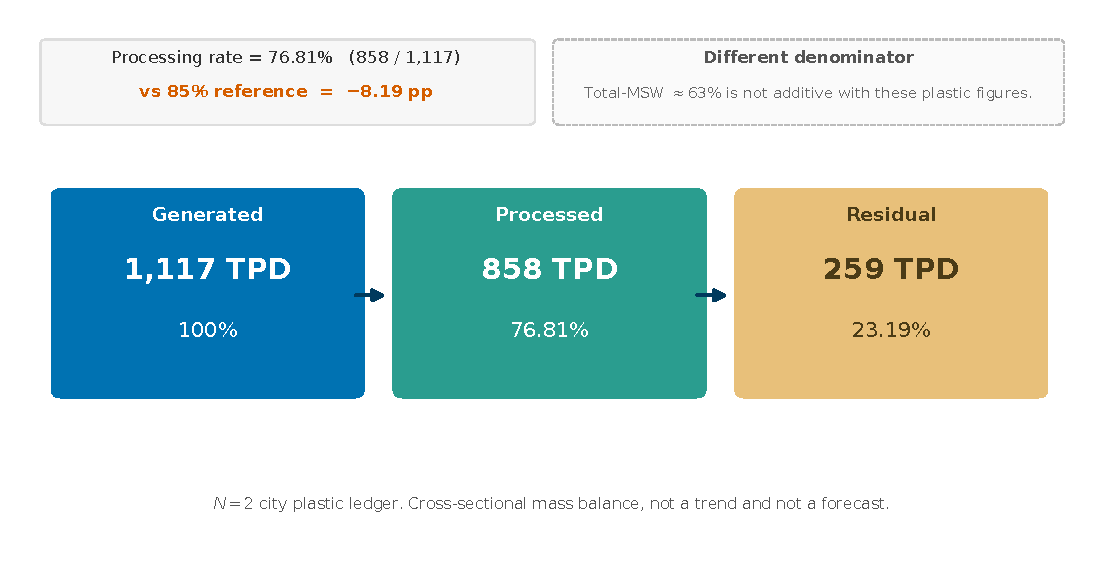
\includegraphics[width=\linewidth,keepaspectratio]{fig4.pdf}
\caption{Plastic mass balance at city scale from DPCC Section~VIII: 1{,}117 TPD generated, 858 TPD processed, 259 TPD arithmetic processing remainder, recorded identically in March and June 2025. The ratio is of two recorded quantities and has no interval. The $\approx$63\% total-MSW figure is a different denominator and is not additive. Cross-sectional ledger, not a trend.}
\label{fig:fig4}
\end{figure}




The same city-scale remainder coexists with heterogeneous infrastructure rather than a simple capacity shortage. Table~\ref{tab:table5} and Figure~\ref{fig:fig5} classify each plant against design capacity: utilization is 58.3\% at Ghazipur, 68.0\% at Tehkhand, 95.8\% at Okhla, and 108.4\% at Bawana --- a 50.1 percentage-point range (CV 28.3\%). Ghazipur and Tehkhand are Underutilized (mixed-waste headroom 347.7 and 340.7 TPD to the 85\% operating band; combined 688.4 TPD). Okhla is High Utilization and is not treated as slack. Bawana is Over-Stressed. Delhi's infrastructure problem is therefore two jobs: relieve Bawana, and fill Ghazipur and Tehkhand up to mixed-waste headroom after availability and compliance checks. The 259 TPD remainder is plastic-specific; the 688.4 TPD headroom is mixed-waste throughput. The two TPD figures remain on separate ledgers. The facility layer is necessary for that reason: without it, the city remainder would be read as a uniform capacity shortage.

Ghazipur was reported non-operational for 108 of 275 days between April and December 2025 \citep{ht_ghazipur_shutdown_2026}, a direction consistent with underutilization. A CPCB affidavit before the National Green Tribunal in February 2026 flagged Bawana for dioxin/furan exceedances and Ghazipur/Tehkhand for effluent-treatment lapses, while identifying Okhla as the only plant meeting all monitored norms \citep{ht_cpcb_affidavit_2026}. Compliance and utilization remain separate instruments; Okhla is retained at High Utilization on the measured 95.8\% rate.



\begin{table}[htbp]
\centering
\caption{WTE facility utilization and benchmark classification}
\label{tab:table5}
\resizebox{\textwidth}{!}{%
\begin{tabular}{L{1.9cm}L{1.9cm}L{1.7cm}L{1.3cm}L{2.1cm}L{1.7cm}L{4.2cm}}
\toprule
\textbf{Facility} & \textbf{Designed capacity} & \textbf{Processing} & \textbf{Util.\ \%} & \textbf{Classification} & \textbf{Mixed-waste headroom to 85\%} & \textbf{Operational interpretation} \\
\midrule
Ghazipur & 1,300 & 757.3 & 58.3 & Underutilized & 347.7 TPD & Direction matches reported 108-day FY2025-26 shutdown \citep{ht_ghazipur_shutdown_2026} \\
Tehkhand & 2,000 & 1,359.3 & 68.0 & Underutilized & 340.7 TPD & CPCB affidavit flags effluent-treatment lapses \citep{ht_cpcb_affidavit_2026} \\
Okhla & 1,950 & 1,867.9 & 95.8 & High Utilization & -- & Not over-stressed; only plant meeting all monitored CPCB norms \citep{ht_cpcb_affidavit_2026} \\
Bawana & 2,000 & 2,167.5 & 108.4 & Over-Stressed & -- & Above designed capacity; CPCB affidavit flags dioxin/furan exceedances \\
\midrule
\multicolumn{7}{l}{Utilization range = 50.1 pp (heterogeneity metric); CV = 28.3\%; combined Ghazipur+Tehkhand mixed-waste throughput headroom to 85\% = 688.4 TPD} \\
\bottomrule
\end{tabular}%
}
\begin{flushleft}
\footnotesize\textit{Note.} Bands: $<$85\% Underutilized; 85--95\% Optimal; 95--100\% High Utilization (conditionally admissible, not slack); $>$100\% Over-Stressed. Source: \citet{dpcc_mpr_2025}, Annexure-5 (facility mixed-waste census snapshot). Headroom is mixed-waste throughput to the 85\% operating band, not plastic-only capacity. External reports are directional context.
\end{flushleft}
\end{table}






\begin{figure}[htbp]
\centering
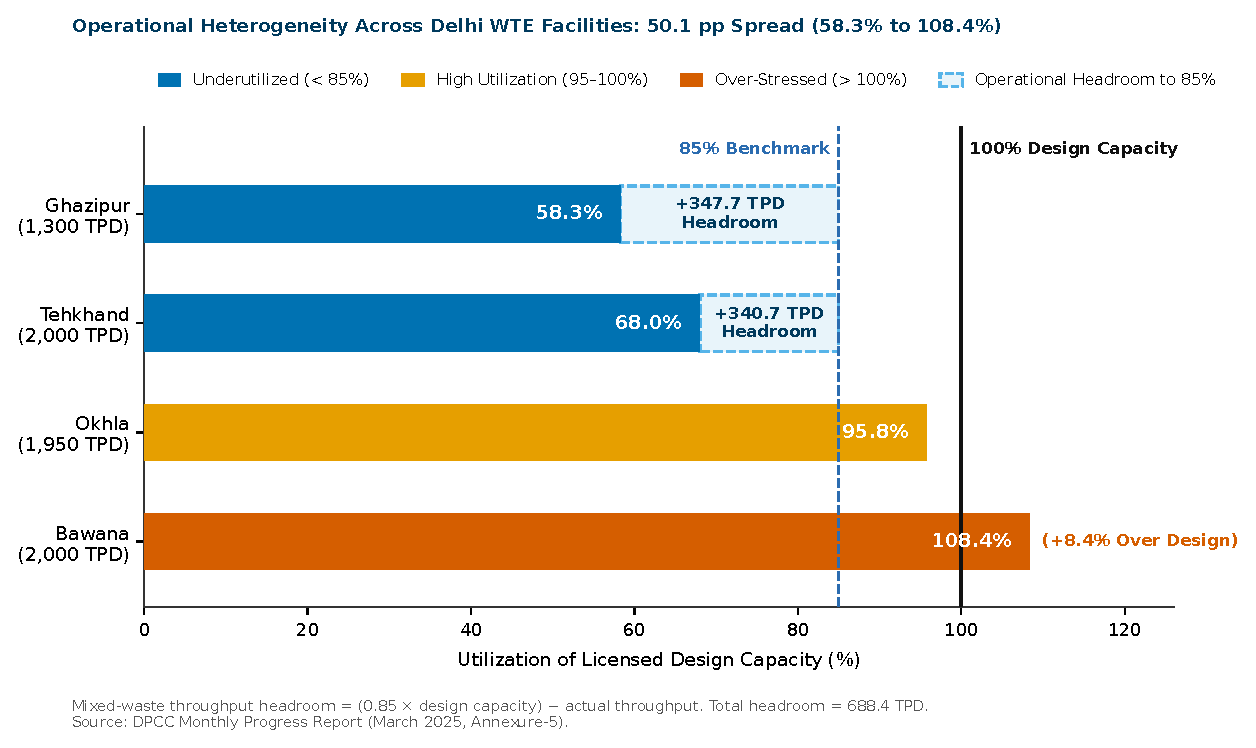
\includegraphics[width=\linewidth,keepaspectratio]{fig5.pdf}
\caption{Four-plant utilization census snapshot. Ghazipur 58.3\% and Tehkhand 68.0\% are underused (mixed-waste throughput headroom 347.7 and 340.7 TPD to 85\%); Okhla 95.8\% is High Utilization and not treated as slack; Bawana 108.4\% is over-stressed. The 50.1 percentage-point range is heterogeneity, not a $p$-value. Source: \citet{dpcc_mpr_2025}, Annexure-5.}
\label{fig:fig5}
\end{figure}




\subsection{Robustness of intervention priorities}
\label{sec:res-robust}

\textbf{Finding.} Global rank stability does not licence every site. \textbf{Quantification.} Weighting tests yield mean Spearman $\rho=0.893$ and mean top-10 overlap 83.3\%. Mean leave-one-out rank displacement is 0.55 positions. The missing-data comparison leaves the recorded top-10 unchanged (Spearman $\rho=1.000$). \textbf{Interpretation boundary.} The high mean rank correlation therefore does not licence universal confidence in the ranking. Stability must be evaluated at the decision-unit level. Only Kamla Nehru Ridge, Kashmere Gate ISBT, and CBD Karkardooma are GREEN (each 8/9 = 88.9\%). DAV School records 9/9 appearance but is AMBER because it is LOO-influential (mean displacement 3.7 positions, maximum 19). Ryan International School is RED (5/9). \textbf{Decision consequence.} Immediate collection spend is licensed only for the three GREEN names; DAV School licences a site investigation; the remaining names are withheld (Table~\ref{tab:table6}; Figure~\ref{fig:fig6}). Kashmere Gate ISBT is not LOO-influential (mean leave-one-out displacement 0.96, maximum 1). DAV School is, because its PVC value is extreme (mean 3.7, maximum 19), not because the record is invalid. PVC-based and percentile-normalized rankings are more method-sensitive than overall burden. The 3-of-58 result is therefore a withholding rule rather than a weak ranking: unstable evidence is not converted into spend.



\begin{table}[htbp]
\centering
\caption{Robustness of locality intervention priorities (appearance-rate registry)}
\label{tab:table6}
\resizebox{\textwidth}{!}{%
\begin{tabular}{L{4.2cm}L{2.2cm}L{2.6cm}L{2.4cm}L{2.4cm}}
\toprule
\textbf{Locality} & \textbf{Top-10 hits} & \textbf{Survival \%} & \textbf{LOO influence} & \textbf{Class} \\
\midrule
Kamla Nehru Ridge & 8/9 & 88.9 & 0.98 (max 2) & GREEN \\
Kashmere Gate ISBT & 8/9 & 88.9 & 0.96 (max 1) & GREEN \\
CBD Karkardooma & 8/9 & 88.9 & 0.95 (max 1) & GREEN \\
DAV School & 9/9 & 100.0 & 3.74 (max 19) & AMBER \\
National Museum & 7/9 & 77.8 & -- & AMBER \\
Shakarpur & 6/9 & 66.7 & -- & AMBER \\
Ryan International School & 5/9 & 55.6 & -- & RED \\
\midrule
\multicolumn{5}{l}{Weighting mean Spearman $\rho$=0.893; mean top-10 overlap=83.3\%; mean LOO displacement=0.55; 3 GREEN} \\
\bottomrule
\end{tabular}%
}
\begin{flushleft}
\footnotesize\textit{Note.} Hits are appearances in the recorded top-10 test (9 weighting/normalization rows). LOO influence is mean (maximum) rank displacement of the remaining localities when that name is removed. Influence is flagged when that mean exceeds 1.0; only DAV School meets that rule. GREEN/AMBER/RED are locality-priority classes only (Table~\ref{tab:robusttests}). Three of 58 names are GREEN.
\end{flushleft}
\end{table}






\begin{figure}[htbp]
\centering
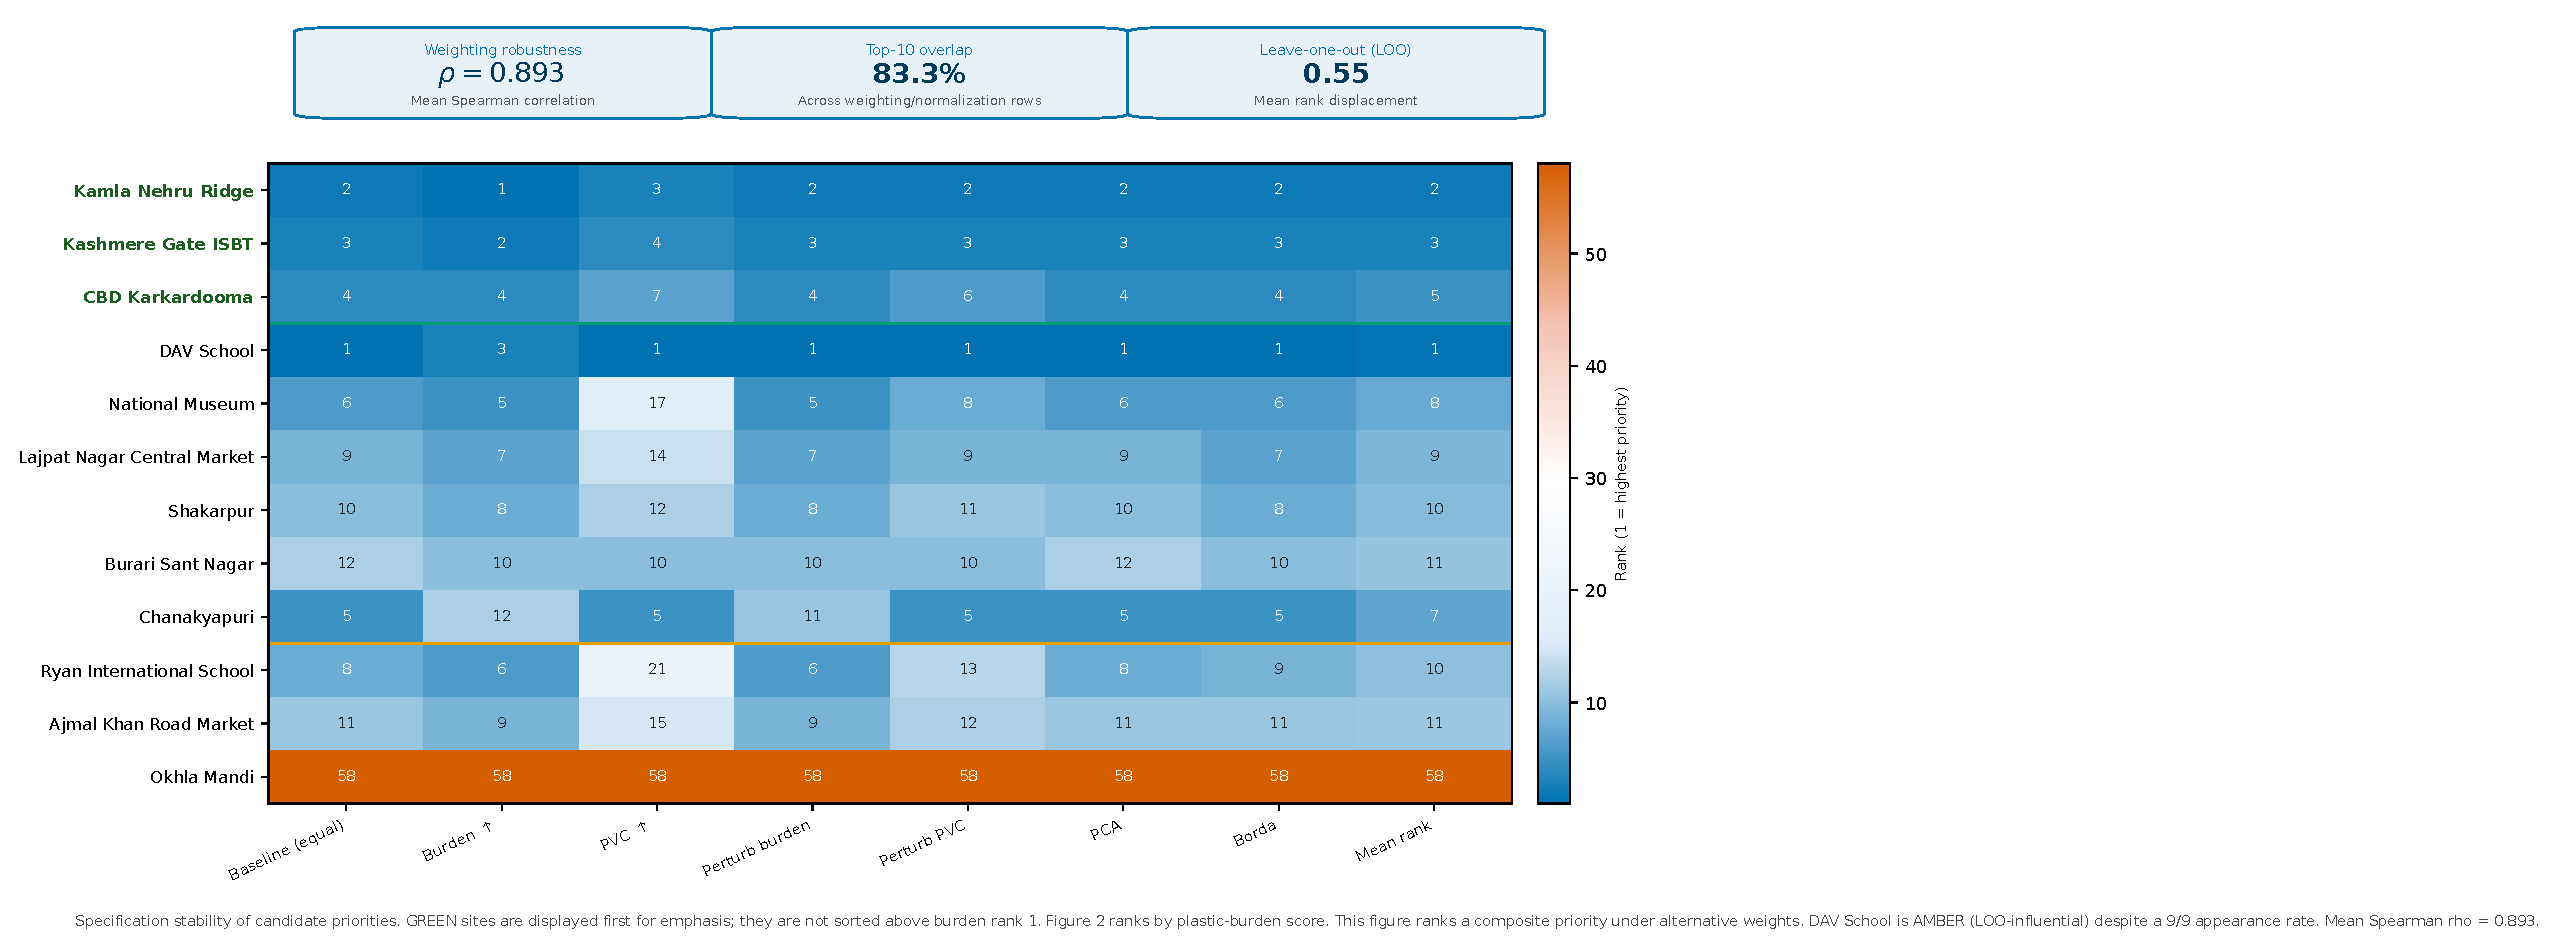
\includegraphics[width=\linewidth,keepaspectratio]{fig6.pdf}
\caption{Specification stability of candidate priorities. GREEN sites (Ridge, Kashmere Gate ISBT, CBD Karkardooma) are displayed first for emphasis; they are not sorted above burden rank 1. Figure~\ref{fig:fig2} ranks by plastic-burden score; this figure ranks a composite priority under alternative weights. DAV School is AMBER because removing it shifts other ranks (mean 3.7, maximum 19), despite a 9/9 appearance rate. Kashmere Gate ISBT remains GREEN: appearance 8/9 and mean leave-one-out displacement 0.96. Weighting $\rho=0.893$; top-10 overlap 83.3\%; LOO 0.55.}
\label{fig:fig6}
\end{figure}




\subsection{Constraint set and evidence-to-intervention screen}
\label{sec:res-routing}

The sequence is evidence $\rightarrow$ eligibility $\rightarrow$ constraint $\rightarrow$ intervention, not evidence $\rightarrow$ intervention. Ridge, Kashmere Gate ISBT, and CBD Karkardooma: observed high burden, robustness survives, eligible localities, collection and segregation intervention. DAV School: PVC spike, LOO influence, not robust enough for a direct programme, site investigation. Ghazipur and Tehkhand: underused relative to design, candidate sinks up to mixed-waste headroom at 85\%; Bawana, over design, is a blocked node; Okhla, at High Utilization, stays in the network as conditionally admissible and is not treated as slack. Combining that classification with locality burden supplies two of the three layers a reverse-logistics network needs: origin demand and destination capacity. Catchments, GPS, and fleets --- the third layer --- are not in the files. The logistics layer is required because a utilization ratio is not a route, and a city shortage is not a haul: origins, candidate sinks, and blocked nodes must be established before a later model assigns flow. Table~\ref{tab:table7} and Figure~\ref{fig:fig7} are therefore a constraint set from which a later capacitated routing model can be solved, not a routing solution itself. Extra kilometres are assumed. MCD's proposed additions at Ghazipur, Okhla, and Tehkhand \citep{nie_mcd_four_plants_2025,toi_tehkhand_expansion_2026,nie_processing_gap_2026} agree in direction with relieving the same imbalance.



\begin{table}[htbp]
\centering
\caption{Reverse-logistics constraint set (not a routing solution)}
\label{tab:table7}
\resizebox{\textwidth}{!}{%
\begin{tabular}{L{3.0cm}L{3.4cm}L{2.4cm}L{2.2cm}L{3.6cm}}
\toprule
\textbf{Illustrative origin} & \textbf{Role in the set} & \textbf{Permitted sink} & \textbf{Assumed extra km} & \textbf{Mixed-waste headroom to 85\%} \\
\midrule
Dwarka Sector-12 & Demand node (scenario) & Tehkhand & 1.2 & 340.7 TPD \\
Azadpur Mandi & Demand node (scenario) & Ghazipur & 1.9 & 347.7 TPD \\
Vikaspuri & Demand node (scenario) & Tehkhand & 3.39 & 340.7 TPD \\
Uttam Nagar & Demand node (scenario) & Tehkhand & 3.39 & 340.7 TPD \\
Burari Sant Nagar & Demand node (scenario) & Ghazipur & 3.57 & 347.7 TPD \\
\midrule
Bawana (facility) & Blocked node (108.4\% observed) & --- & --- & Load withheld \\
Okhla (facility) & High Utilization (95.8\%) & --- & --- & Not treated as slack \\
\bottomrule
\end{tabular}%
}
\begin{flushleft}
\footnotesize\textit{Note.} Origins are scenario demand nodes; extra km are assumed round-trips. Sink headroom is mixed-waste throughput to the 85\% operating band from \citet{dpcc_mpr_2025}, Annexure-5; it is not the city plastic remainder of 259 TPD in Table~\ref{tab:table4}. Direction matches MCD capacity notices \citep{nie_mcd_four_plants_2025,toi_tehkhand_expansion_2026}.
\end{flushleft}
\end{table}






\begin{figure}[htbp]
\centering
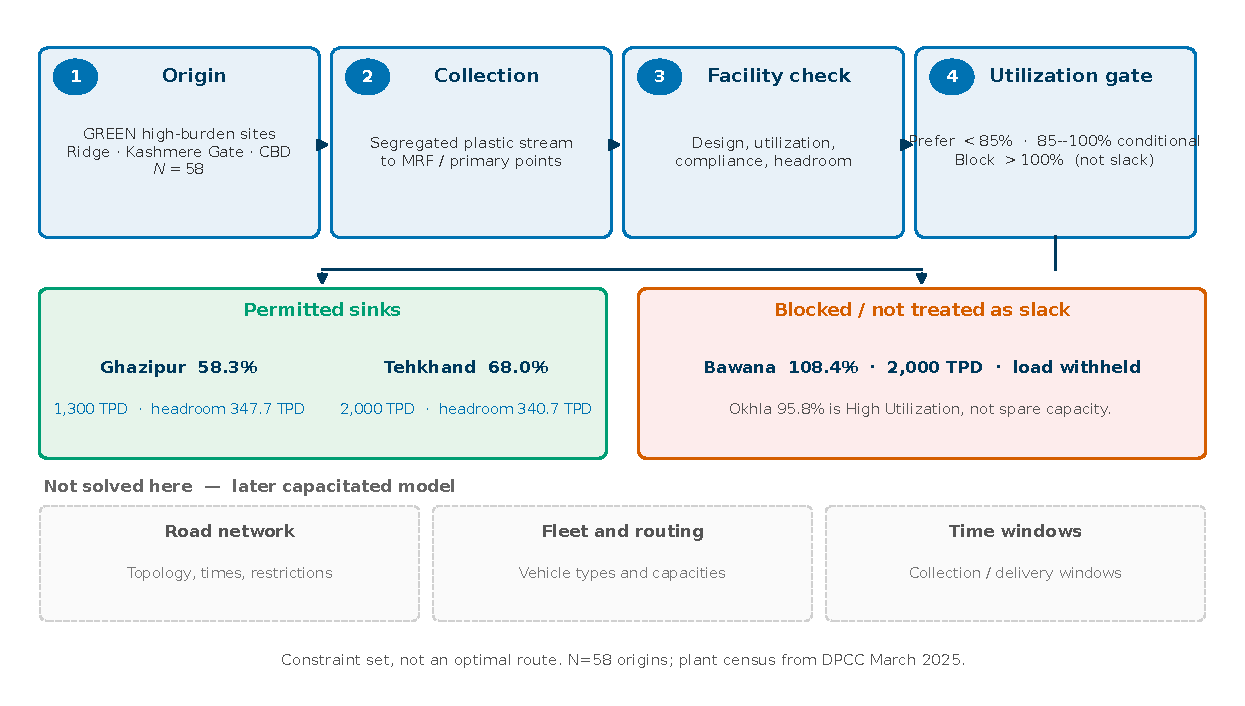
\includegraphics[width=\linewidth,keepaspectratio]{fig7.pdf}
\caption{Feasibility layer of a later reverse-logistics model: a constraint set, not an optimal route. Preferred sinks: plants below 85\% of design, up to mixed-waste throughput headroom. Conditionally admissible: 85--100\% of design (Okhla 95.8\% High Utilization, not slack). Blocked: above 100\% of design (Bawana). Road network, fleet, and time windows are not solved here.}
\label{fig:fig7}
\end{figure}




Table~\ref{tab:table8} and Figure~\ref{fig:fig8} are the decision screen for those layers. A robust locality-burden finding is never presented with the same confidence as a PVC investigation flag or a two-point processing ledger. High-burden GREEN localities warrant direct collection and segregation investment; the DAV School PVC concentration warrants a site investigation; elevated PET or PP prevalence warrants an assessment of MRF access; the 259 TPD remainder warrants a plastic line in the municipal ledger; and the Ghazipur/Tehkhand headroom paired with Bawana's over-stress warrants utilization rebalancing before, or alongside, new-capacity investment. Supplementary Figure~S1 records the triangulation rule: measurements, official numbers used as context, and inference remain three distinct evidence classes.



\begin{table}[htbp]
\centering
\caption{Evidence-to-intervention decision table}
\label{tab:table8}
\resizebox{\textwidth}{!}{%
\begin{tabular}{L{2.2cm}L{3.4cm}L{2.6cm}L{3.2cm}L{3.4cm}}
\toprule
\textbf{Evidence object} & \textbf{Finding} & \textbf{Evidence status} & \textbf{Licensed intervention} & \textbf{Explicitly not licensed} \\
\midrule
Material burden & Up to 30.49\% ($N=58$); Ridge 30.49\%, Kashmere Gate 30.25\%, CBD 22.68\% & ROBUST PRIORITY & Collection/segregation at robust high-burden sites, with small-sample flags & Citywide processing failure from locality shares \\
PVC & Max 15.43\% (DAV School); mean 1.65\% & INVESTIGATION & Site-specific PVC investigation & Citywide PVC restriction or a PET recycling rate analogue \\
PET & Mean 23.60\%; Kashmere Gate 83.68\% & DESCRIPTIVE & MRF access/throughput and capture assessment & PET recycling rate or locality circularity \\
PP & Mean 2.79\% & DESCRIPTIVE & EPR-linked recovery-pathway assessment & E-commerce origin or a performance score \\
Processing ledger & 858 of 1,117 TPD; remainder 259 TPD & TWO-RECORD LEDGER & Plastic fate/ledger investigation & Citywide recycling-efficiency claim or a trend \\
WTE utilization & 58.3--108.4\%; 50.1 pp range & CENSUS SNAPSHOT & Scenario-based load rebalancing: fill Ghazipur/Tehkhand; relieve Bawana & Optimal routing; treating Okhla as slack \\
Bawana over-stress & 108.4\% of design & CENSUS SNAPSHOT & Operational-relief assessment & Proven cause of emissions non-compliance \\
Spatial concentration & High--high: Kamla Nagar Market, Tis Hazari; Ridge and Kashmere Gate not classified & LISA-CONFIRMED & Zone plans for confirmed hotspots; site lifting at isolated generators & High-burden name as hotspot name \\
\bottomrule
\end{tabular}%
}
\begin{flushleft}
\footnotesize\textit{Note.} Evidence status names the type of supporting object. GREEN/AMBER/RED are reserved for locality-priority classes (Tables~\ref{tab:robusttests} and~\ref{tab:table6}) and are not reused as chips for plants, ledgers, or clusters. Read with Table~\ref{tab:licensed}.
\end{flushleft}
\end{table}






\begin{figure}[htbp]
\centering
\caption{Evidence-to-intervention decision screen. Status chips name the evidence object. Corresponds to Table~\ref{tab:table8}. Do not transfer evidence beyond its measurement scale without validation.}
\label{fig:fig8}
\resizebox{\textwidth}{!}{%
\begin{tabular}{L{2.6cm}L{3.4cm}L{3.3cm}L{5.4cm}}
\toprule
\textbf{Evidence object} & \textbf{Evidence status} & \textbf{Licensed} & \textbf{Not licensed} \\
\midrule
1.\ Locality burden & \statuschip{chipgreen}{ROBUST PRIORITY} & Collection at Ridge, Kashmere Gate, CBD & Export of these ranks to other cities or years \\
2.\ PVC & \statuschip{chippurple}{INVESTIGATION} & Site investigation at DAV School & Citywide PVC restriction \\
3.\ PET / PP & \statuschip{chipgrey}{DESCRIPTIVE} & MRF access and capture assessment & Equating PET share with a recycling rate \\
4.\ City processing & \statuschip{chipbrown}{TWO-RECORD LEDGER} & Plastic line and fate investigation & Trend or forecast from $N=2$ \\
5.\ WTE utilization & \statuschip{chipnavy}{CENSUS SNAPSHOT} & Relieve Bawana; fill Ghazipur/Tehkhand & Treating Okhla as slack \\
6.\ Spatial clusters & \statuschip{chipblue}{LISA-CONFIRMED} & Zone plans for confirmed clusters; site lifting at isolated generators & High-burden name as hotspot name \\
\bottomrule
\end{tabular}%
}
\begin{flushleft}
\footnotesize\textit{Note.} GREEN/AMBER/RED are reserved for locality-priority robustness classes (Table~\ref{tab:table6}). Other labels identify the evidence type and are not robustness grades.
\end{flushleft}
\end{figure}




%% ====================================================================
\section{Discussion}
\label{sec:discussion}

A locality share, a city processing rate, and a plant-utilization spread can all be printed as percentages. They cannot all support the same action. Collection contracts are priced at the first, dashboards usually quote the second, and intake is decided at the third. Treating them as interchangeable is evidence-scale mismatch (Table~\ref{tab:mismatch}). Each subsection below follows the same rhythm: the finding, why it may arise, how prior work sits beside it, the business and environmental implication, and the decision that the evidence can licence (Table~\ref{tab:licensed}).

\subsection{Concentrated burden and the spatial unit of action}

A named tail is found, not a city average. Kamla Nehru Ridge (30.49\%) and Kashmere Gate ISBT (30.25\%) occupy the extreme upper end of the $N=58$ sample; CBD Karkardooma follows at 22.68\% (Table~\ref{tab:table2}; Figure~\ref{fig:fig2}). A plausible reading is throughput at a transit hub and visitor litter at a mixed ridge site with a very small sample; those mechanisms are not directly observed. Earlier Delhi characterization work already showed that resin shares vary by area type \citep{delhi_plastic_characterization_study}, and CPCB reporting used city or pilot-city averages as the unit \citep{cpcb_60cities_2015,cpcb_sop_pwm_2024}. Variation is therefore already established. Local Moran's I supplies the missing unit of action (Table~\ref{tab:table3}; Figure~\ref{fig:fig3}): Kamla Nagar Market and Tis Hazari Court are high--high clusters, so the object is a zone; Ridge and Kashmere Gate are not classified, so the object is a site. Kumar, Choudhary and Mathur drew the hotspot/outlier distinction for municipal solid waste in Kota \citep{ieam_kota_landuse_msw_2026}; it is used here with the restriction that no cluster label is assigned where LISA is not significant.

The business and environmental implication is a crew assignment, not a public announcement. The Kashmere Gate site records a PET-rich sampled stream, plausibly reflecting the site's transit and packaged-consumption context; the Kamla Nagar commercial site records a statistically confirmed high--high cluster. Residents on average-priced beats may pay for a service that can miss those nodes. Material that remains outside the documented collection and processing pathway can increase the risk that unmanaged waste enters uncontrolled environmental pathways. MCD's source-segregation roadmap illustrates why a named beat matters: a citywide target does not assign a truck to an ISBT platform \citep{toi_segregation_roadmap_2026,nie_segregation_failed_2026}. The decision that follows is two contract clauses: site lifting at the three GREEN high-burden generators, and zone attention only where a high--high cluster is confirmed. The result is therefore not merely that plastic burden varies spatially. It is that the spatial unit of intervention cannot be inferred from burden alone: isolated high-burden generators and statistically coherent clusters require different operational responses.

\subsection{Composition as prevalence, not circularity}

A mix is found, not a recycling rate. Composition is an input to circularity, not evidence of circularity. HDPE/LDPE leads (mean 53.24\%), PET follows (mean 23.60\%), and PVC is rare on average (1.65\%) yet spikes to 15.43\% at DAV School (Table~\ref{tab:table2}). Kashmere Gate ISBT is PET-rich (83.68\% of plastic); Shakarpur is HDPE/LDPE-rich (95.28\%). A plausible reading is use-context: bottled drinks at a transit hub; institutional film or packaged goods at a school. Hossain and colleagues argued that India's circular-economy architecture is stronger on rules than on source-specific recovery \citep{haque_plastic_waste_india_2022}; CPCB's SOP reported a higher PP share under a different categorization \citep{cpcb_sop_pwm_2024}. Frame dependence explains the mismatch. It does not support the inference that sampled PET is recovered PET.

PET prevalence can justify capture assessment, MRF throughput assessment, or an EPR audit; it cannot establish recovery. PP prevalence may inform packaging investigations, but e-commerce origin is not observed. National reporting of 20.7 million tonnes of plastic packaging recycled since 2022 records compliance obligations at Union scale \citep{dte_epr_recycled_2026,cpcb_pwm_amendment_2026,pib_plastic_waste_2025}, but that reporting has no locality identifier. The decision that follows is to contract MRF throughput where PET is prevalent and to inspect DAV School rather than to impose a territory-wide ban. Prevalence is left in the prevalence column; the PVC spike is labelled AMBER/LOO rather than treated as a citywide policy.

\subsection{A city-scale gap that cannot diagnose the network}

A plastic-specific remainder is found from the two recorded quantities in Table~\ref{tab:table4} and Figure~\ref{fig:fig4}. The processed share is about 77\%. That quotient has no interval. Incomplete source segregation and incomplete capture are a plausible reading, and independent MCD reporting continues to flag both \citep{nie_segregation_failed_2026,toi_segregation_roadmap_2026}. The Economic Survey's total-MSW shortfall of about 63\% points in the same broad direction on a different denominator \citep{delhi_eco_survey_2026,nie_mcd_four_plants_2025}. Generic WTE reviews and city-scale slides say processing is incomplete; they do not name which node is incomplete \citep{sciencedirect_wte_india_review_2014,mcd_swm_ppt}.

Operationally the 259 TPD is a ledger line, not a plant diagnosis. A citywide processing ratio is therefore a system-level warning signal, not a diagnosis of where the operational bottleneck lies. Combined Ghazipur--Tehkhand headroom of 688.4 TPD cannot close that argument, because it is mixed-waste throughput to an 85\% benchmark. The decision that follows is to record a plastic line next to the total-MSW line and to commission a fate study for the remainder. To locate the bottleneck, the evidence must move from city scale to facility scale.

\subsection{Facility imbalance and confirmed operating evidence}

Facility-level evidence changes the interpretation of the citywide gap. Simultaneous slack and tightness are found across the four-plant census in Table~\ref{tab:table5} and Figure~\ref{fig:fig5}. Underutilized plants and overloaded plants coexist. Ghazipur's reported 108-day FY2025--26 shutdown is an availability constraint; Bawana's over-stress may reflect an unobserved catchment; Okhla's high utilization is an operating ratio rather than a compliance certificate \citep{ht_ghazipur_shutdown_2026,ht_cpcb_affidavit_2026}. Downtime, stack chemistry, and throughput-to-capacity remain different instruments. Generic WTE technology reviews stop before a four-plant census is joined to named origins \citep{sciencedirect_wte_india_review_2014,springer_msw_wte_india_overview_2017}.

The city-scale gap therefore splits into two jobs. Relieving Bawana is an availability and compliance problem; filling Ghazipur and Tehkhand is an intake-and-logistics problem, up to mixed-waste headroom and after chimney, Graded Response Action Plan, and effluent constraints. Capacity policy should distinguish redistribution from expansion. WTE operators, insurers, logistics contractors, and residents near an over-run grate are the exposed parties; a CPCB dioxin/furan flag at Bawana is independent context rather than an emission estimate from these files. MCD expansion notices agree in direction \citep{nie_mcd_four_plants_2025,toi_tehkhand_expansion_2026}. The decision that follows is to budget those two jobs on two lines and to keep Okhla in the network as High Utilization rather than as a slack sink.

\subsection{Robustness as a withholding rule}

A priority is only as defensible as the specification under which it survives. A gate is found, not a league table. Two properties are scored separately, which is why Kashmere Gate ISBT and DAV School do not receive the same licence. Appearance stability measures whether a locality remains in the recorded top-10 when weights and scaling change. Leave-one-out influence measures the effect of removing that locality on the ranking of the remaining names. GREEN requires both. Kashmere Gate ISBT satisfies both (8/9 appearance; mean displacement 0.96). DAV School satisfies only the first (9/9 appearance; mean displacement 3.7) and is therefore AMBER: licensed for site investigation, not for a multi-site PVC programme. Weighting mean Spearman $\rho=0.893$, mean top-10 overlap 83.3\%, mean leave-one-out displacement 0.55; three GREEN burden names --- Kamla Nehru Ridge, Kashmere Gate ISBT, CBD Karkardooma --- and DAV School held at AMBER despite a 100\% appearance rate (Table~\ref{tab:table6}; Figure~\ref{fig:fig6}). The high mean rank correlation therefore does not licence universal confidence in the ranking. Global stability metrics can conceal local instability. Overall burden ranking is less method-sensitive than PVC-driven or percentile-scaled ranking; DAV School moves other ranks because its PVC value is extreme. The Kota study used more than one spatial estimator to confirm clusters \citep{ieam_kota_landuse_msw_2026}. Composition and WTE papers rarely test whether a priority list is an artefact of scaling.

The same 3-of-58 result can be read as a fragile ranking or as a conservative gate. Both readings are licensed by the numbers. The first reading warns against treating the untested top-10 as a programme. The second is the one used for spend: only the three surviving names are listed for immediate collection, and DAV School is sent for inspection rather than for a citywide PVC rule. Robustness should therefore be treated as a property of the intervention decision, rather than as an optional sensitivity appendix. Once urban local bodies select pilots, an untested ranking becomes a budget \citep{cpcb_pwm_amendment_2026}. Rank stability is treated as part of what a priority is, following the older multiple-criteria and sensitivity literature \citep{belton_stewart_2002,saltelli_sensitivity_2008}, not as a boast that the method is robust.

\subsection{Supply-chain translation and the theoretical join}

A constraint set is found from the facility-wise utilization results: high-burden localities as demand nodes; Ghazipur and Tehkhand as candidate sinks up to mixed-waste headroom; Bawana blocked; Okhla High Utilization (Table~\ref{tab:table7}; Figure~\ref{fig:fig7}). That is the supply-chain translation this paper can defend. The contribution is not an optimized route. It is an evidence-constrained set of origins, candidate sinks and capacity constraints from which an optimization model can subsequently be constructed. Generic WTE technology reviews and spatial hotspot studies each stop at one of those two layers \citep{sciencedirect_wte_india_review_2014,ieam_kota_landuse_msw_2026}. A contractor can scope a pilot from this set. A timetable cannot be run from it. The decision that follows is to provide a later routing team with this file so that slack plants are not reopened as unresolved design questions.

The empirical join is Table~\ref{tab:contribution}. The claim stated in Section~\ref{sec:introduction} is demonstrated rather than restated. What can be reused is the sequence of layers, not these ranks (Section~\ref{sec:transfer}). A city with a locality composition file, a processing ledger, a plant census, and a specification registry can run the same sequence. It cannot import Kamla Nehru Ridge or the two-point processing ratio.



\begin{table}[htbp]
\centering
\caption{How disconnected literature streams are joined into an evidence-linked decision architecture}
\label{tab:contribution}
\resizebox{\textwidth}{!}{%
\begin{tabular}{L{2.8cm}L{3.0cm}L{3.2cm}L{3.0cm}L{3.4cm}}
\toprule
\textbf{Conventional sequence} & \textbf{Evidence unit kept separate} & \textbf{Diagnosis produced} & \textbf{Gate applied} & \textbf{Intervention licensed} \\
\midrule
Composition surveys \citep{delhi_plastic_characterization_study,cpcb_60cities_2015,cpcb_sop_pwm_2024} & Locality burden and resin mix ($N=58$) & Named tail: Ridge 30.49\%, Kashmere Gate 30.25\%; PET as prevalence (23.60\%); PVC scored at DAV School 15.43\% & Priority status varies by locality; Ridge, Kashmere Gate ISBT and CBD Karkardooma survive the robustness gate. PVC at DAV School is held AMBER (LOO) & Site lifting at GREEN generators; site inspection at DAV School, not a city PVC ban \\
Spatial MSW analysis \citep{ieam_kota_landuse_msw_2026} & Local Moran's I only where $p<0.05$ & High--high: Kamla Nagar Market, Tis Hazari; Ridge and Kashmere Gate unclassified & High-burden name $\neq$ hotspot name & Zone plan for confirmed clusters; site lifting for isolated generators \\
City MSW aggregates \citep{delhi_eco_survey_2026,mcd_swm_ppt} & Plastic ledger (two records), distinct from $\approx$63\% total MSW & 858 of 1,117 TPD processed; 259 TPD remainder & Remainder not mixed with mixed-waste headroom & Plastic line in the municipal ledger; fate study \\
WTE technology reviews \citep{sciencedirect_wte_india_review_2014,springer_msw_wte_india_overview_2017} & Four-plant census from \citet{dpcc_mpr_2025} & 50.1 pp spread; Ghazipur/Tehkhand underused; Okhla 95.8\% High Utilization; Bawana 108.4\% over-stressed & Headroom kept as mixed-waste throughput; Okhla not treated as slack & Two jobs: relieve Bawana; fill Ghazipur/Tehkhand \\
Policy targeting without specification testing \citep{haque_plastic_waste_india_2022,cpcb_pwm_amendment_2026} & Policy frameworks specify obligations but do not, in the cited evidence, establish locality-level priority stability. This study introduces a specification registry (72 rows) before immediate intervention & $\rho=0.893$; top-10 overlap 83.3\%; LOO 0.55; three of 58 names survive & Immediate spend withheld from method-sensitive names & Immediate spend only on Ridge, Kashmere Gate, CBD Karkardooma \\
\bottomrule
\end{tabular}%
}
\begin{flushleft}
\footnotesize\textit{Note.} Column sequence is the join demonstrated after the results. Ranks are not exported; the architecture is. Read with Tables~\ref{tab:mismatch}, \ref{tab:licensed} and~\ref{tab:table8}.
\end{flushleft}
\end{table}




%% ====================================================================
\section{Implications}
\label{sec:implications}

The preceding section established what the measurements can support. This section states what that support implies for urban circularity decision-making, for operational allocation, and for policy and environmental scope.

\subsection{Theoretical implication: circularity decisions need evidence-type preservation}

The theoretical implication extends beyond plastic waste. Urban sustainability decisions routinely combine indicators generated at different spatial and causal levels. A citywide average can describe system performance while remaining uninformative about the location of intervention; a material-composition indicator can describe prevalence while remaining silent on recovery; and a statistically stable aggregate ranking can conceal instability in individual decision units. The architecture developed here addresses that general problem by requiring evidence to retain its measurement unit until a defensible transfer condition is satisfied (Table~\ref{tab:mismatch}). The scientific object is the admissible hand-off between those evidence objects, not a new estimator for any one of them. It is not a claim of a general framework proven for all urban circularity systems. Hossain et al.\ and the CSIRO review already located India's circular-economy weakness at source-specific recovery \citep{haque_plastic_waste_india_2022,csiro_ce_policy_india_2021}. If recovery is inferred from composition, later claims about EPR effectiveness rest on the wrong variable. If plant balance is inferred from a city rate, later claims about capacity shortage rest on the wrong spatial unit. If a rank that fails a specification test is still called a priority, later claims about targeting rest on an unstable object. Rank stability belongs inside the definition of a priority the way multiple estimators belong inside the definition of a hotspot \citep{ieam_kota_landuse_msw_2026,belton_stewart_2002,saltelli_sensitivity_2008}. That is why this paper does not build a composite circularity index, and why Table~\ref{tab:contribution} is an architecture join rather than a weighted score.

\subsection{Managerial and operational implication: allocation should be conditional on evidence stability}

A finding becomes operationally useful only when its spatial and evidentiary scope matches the decision to which it is applied. For the municipal corporation, spend should follow names that survive perturbation: a transit hub as a generator site, a confirmed high--high cluster as a zone. Average-priced contracts that ignore that split can transfer cost onto low-intensity streets or high-throughput hubs, and can increase the risk that unmanaged material enters uncontrolled environmental pathways. An institutional PVC spike is a site inspection, not a territory-wide restriction. The licensed next step is a handling assessment that determines whether chlorinated resin is entering thermal treatment and, if so, whether diversion is warranted.

For producers, brand owners, and recyclers the usable product is an audit list. EPR creates compliance obligations and associated consequences for non-compliance \citep{cpcb_pwm_amendment_2026,pib_plastic_waste_2025}. Reporting that collapses composition, processing and facility utilization into a single circularity claim risks overstating system performance. Additional MRF throughput may be contracted where PET is prevalent, and take-back may be considered where PP packaging is prevalent. That PP reading is interpretive; e-commerce origin was not measured. Firms that require a Delhi circularity claim for investors should commission capture rates, not reprint a composition mean.

For WTE operators and logistics contractors the usable product is two jobs and a feasibility file. Relieving an over-design plant is an availability and compliance problem; filling slack plants is an intake-and-logistics problem. The environmental stake is coincident risk, not proven causation: the plant that is over-stressed is also the plant independently flagged for dioxin/furan \citep{ht_cpcb_affidavit_2026}. Rebalancing is a way not to add load to that coincidence. It is not a certified emissions offset. Okhla remains High Utilization, not slack. Demand nodes, blocked nodes, candidate sinks, and assumed extra kilometres are enough to scope a pilot and not enough to run a fleet.

\subsection{Policy and environmental implication: intervention scope should match measurement scope}

Targeted collection and segregation at surviving names could improve capture opportunity and may reduce the chance that material remains outside the documented pathway. Those links are stated as opportunities, not as measured pollution reductions. Management is not certified from one efficiency number. These NCT ranks are not transferable to Noida or Gurugram. A dashboard should not relabel prevalence as recycling potential.

The transferable contribution is procedural rather than geographic. The absence of multi-city validation limits claims about empirical transferability, but it does not preclude evaluation of the architecture as a decision grammar. The transferable object is the sequence of evidence checks and hand-off conditions; the Delhi-specific values remain non-transferable. That distinction is deliberate: validation of the architecture across cities is a separate empirical question requiring comparable locality, processing, facility, and governance data. A single-city demonstration is still informative here because Delhi is a stringent test: the architecture has to reconcile heterogeneous locality composition, spatial association, city-level processing records, and facility-level utilization without collapsing their denominators or units. Any city possessing locality-level composition, spatial coordinates, city processing records and facility utilization data can implement the sequence: characterize $\rightarrow$ test spatial concentration $\rightarrow$ diagnose processing $\rightarrow$ classify infrastructure $\rightarrow$ test priority stability $\rightarrow$ license intervention $\rightarrow$ optimize logistics only when network data are available. The numerical thresholds, locality rankings and facility headroom reported here remain Delhi-specific. Other cities could apply the same sequence to food-waste recovery, e-waste collection, construction and demolition waste, textile-waste systems, or municipal recycling more broadly. That is a statement about transferable decision discipline, not about empirical validation outside Delhi NCT.

%% ====================================================================
\section{Conclusions}
\label{sec:conclusion}

This study shows that urban plastic circularity cannot be reliably inferred by collapsing locality burden, material prevalence, city processing and facility utilization into a single indicator. An evidence-linked decision architecture is developed, and its application in Delhi NCT is demonstrated. The architecture produces typed decision permissions, not a citywide circularity score.

The empirical demonstration is specific to the sampled frame. Across 58 complete-resin localities, burden ranged from 1.98\% to 30.49\%; Kamla Nehru Ridge and Kashmere Gate ISBT occupy the upper tail but are not LISA hotspots, whereas Kamla Nagar Market and Tis Hazari Court are significant high--high clusters. City processing is 858 of 1,117 TPD (76.81\%), a two-record ledger. Plant utilization spans 58.3--108.4\%. Only three of 58 names survive the robustness gate ($\rho=0.893$; 83.3\% top-10 overlap).

The operational contribution is the sequence from evidence through robustness to licensed intervention and logistics constraints. Composition remains a prevalence observation until capture is measured. The city processing ratio remains a ledger warning until plants are classed. High local burden remains a site candidate until clustering and specification tests are read. Origins and utilization classes supply a constraint set for later routing, not a solved timetable.

The limits are the next measurements: a non-probability locality frame; two city records; one facility snapshot; no capture or recovery rates; no GPS, fleet, or cost files; Delhi NCT only. Comparable NCR sampling and a longer plastic series would be required before ranks or ledgers travel. Until those files exist, the claims above stay inside the design that produced them. The broader contribution is a decision grammar in which evidence is not allowed to travel beyond the spatial, material or operational scale at which it was measured without an explicit validation step. The Delhi values remain city-specific; the sequence of checks and hand-off conditions is the reusable object.

\section*{Supplementary information}

\noindent\textit{Supplementary Figure S1.} Triangulation of measurements, official reports, and inference. The three classes are linked as context, convergence, or not comparable. Different denominators prevent numerical comparison: the $\approx$63\% total-MSW rate and the two-point plastic ratio may both be true without either confirming the other.

\begin{center}
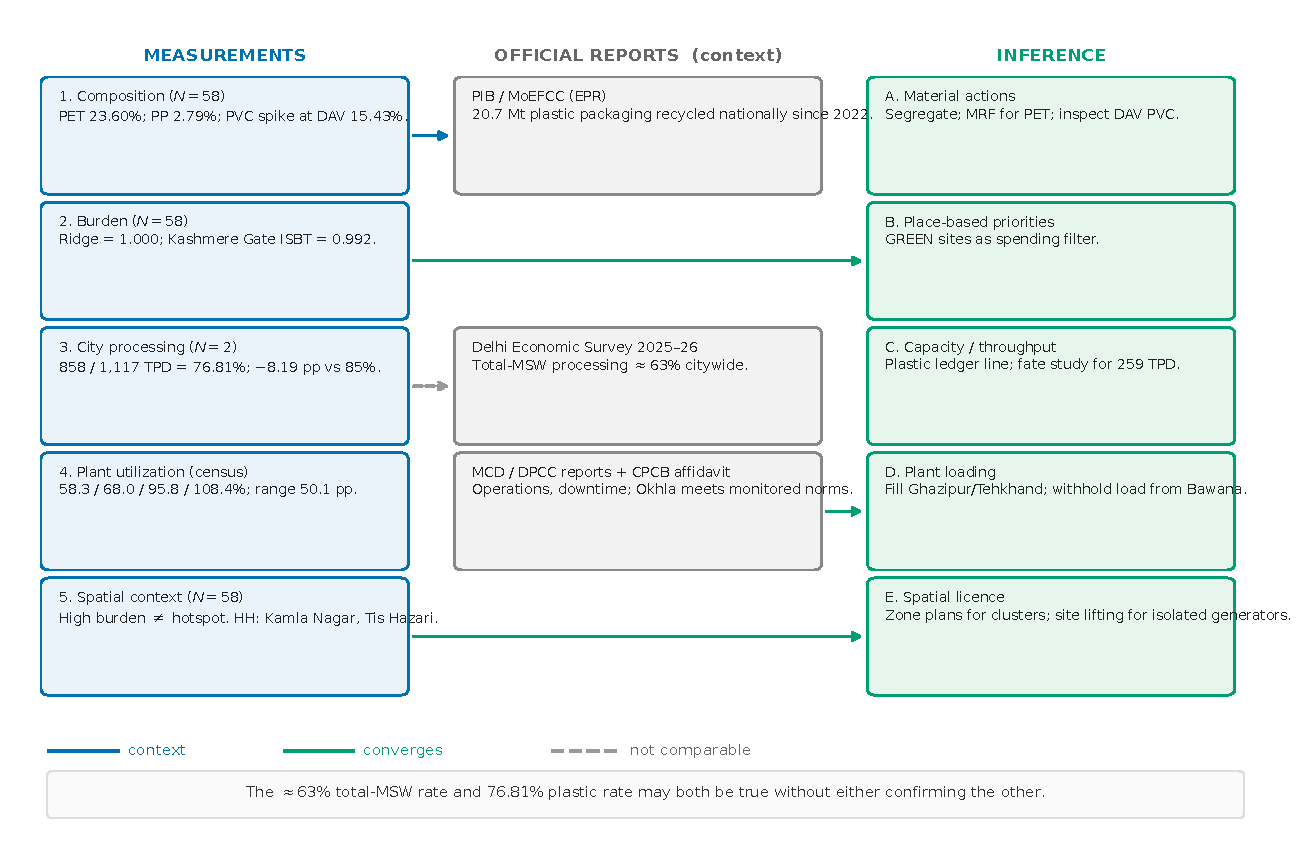
\includegraphics[width=\linewidth,keepaspectratio]{fig9.pdf}
\end{center}

% After any citation or .bib change, delete main.aux and main.bbl and recompile:
%   pdflatex main && bibtex main && pdflatex main && pdflatex main
% Deleting main.bbl is required so older ``Retrieved from https://doi.org/ ... doi:'' lines are not reused.
\bibliographystyle{apacite}
\bibliography{references}

\end{document}

